\documentclass[11pt,a4paper,fontset=fandol]{ctexart}
\usepackage[margin=2.15cm]{geometry}
\usepackage{amsmath,amssymb,booktabs,longtable,array,multirow}
\usepackage{xcolor,enumitem,caption,listings,tikz,fancyhdr}
\usepackage[unicode,colorlinks,linkcolor=blue!45!black,urlcolor=blue!45!black,citecolor=blue!45!black]{hyperref}
\usetikzlibrary{arrows.meta,positioning,calc}
\setmonofont{DejaVu Sans Mono}[Scale=0.82]
\captionsetup{font=small,skip=4pt}
\setlist{itemsep=0.25em,topsep=0.35em,leftmargin=1.7em}
\lstset{
  language=C,
  basicstyle=\ttfamily\footnotesize,
  keywordstyle=\color{blue!55!black}\bfseries,
  commentstyle=\color{green!40!black},
  frame=single,
  framerule=0.35pt,
  rulecolor=\color{black!40},
  columns=fullflexible,
  keepspaces=true,
  showstringspaces=false,
  breaklines=true,
  breakatwhitespace=false,
  tabsize=2,
  morekeywords={reg,ptr_reg},
  xleftmargin=0.4em,
  xrightmargin=0.4em,
  aboveskip=0.6em,
  belowskip=0.4em
}
\pagestyle{fancy}
\fancyhf{}
\fancyhead[L]{\small CacheLab 2026 Part B 分析手册}
\fancyhead[R]{\small\thepage}
\renewcommand{\headrulewidth}{0.3pt}
\setlength{\headheight}{14pt}
\emergencystretch=3em
\hbadness=10000
\newcommand{\code}[1]{\texttt{#1}}
\newcommand{\mreg}{\mathit{miss}_{\mathrm{reg}}}
\newcommand{\mc}{\mathit{miss}_{\mathrm{cache}}}
\title{\textbf{CacheLab 2026 Part B 分析手册}\\[0.4em]
\large 三个 GEMM case 的寄存器分块、cache 映射与缺失分解}
\author{供实验报告的 Part B 使用。读完后应能自己写下三个 case，手册不代替报告正文。}
\date{}

\begin{document}
\maketitle
\thispagestyle{fancy}

\begin{center}
\small
\setlength{\tabcolsep}{5pt}
\begin{tabular}{@{}lrrrr@{}}
\toprule
case & $\mc$ & $\mreg$ & latency & 加速比\\
\midrule
case1，$16\times16\times16$ & $496$ & $2304$ & $9744$ & $8.2438$\\
case2，$32\times32\times32$ & $3200$ & $17408$ & $65408$ & $9.2808$\\
case3，$27\times41\times27$ & $5003$ & $14013$ & $89058$ & $6.8892$\\
\bottomrule
\end{tabular}
\end{center}

\noindent 加权加速比的精确值是 $8.0131$。满分线是 $W=8$，这里 $W>8$，得分率被截断为 $1$，百分制性能分是 $100$。

\noindent 上表每一个整数都来自仓库评测脚本 \code{python3 test/gemm\_test.py}，并与 \code{csim-ref -s 5 -E 1 -b 4} 的输出一致。四位小数是评测脚本的打印格式。精确比值是
\[
\frac{80328}{9744}=8.243842\ldots,\quad
\frac{607040}{65408}=9.280821\ldots,\quad
\frac{613542}{89058}=6.889240\ldots,
\]
加权
\[
W=0.3\cdot\frac{80328}{9744}+0.3\cdot\frac{607040}{65408}+0.4\cdot\frac{613542}{89058}=8.01309557\ldots,
\]
脚本印成 $8.0131$。$(W-1)/(8-1)>1$，所以性能分是 $100$ 而不是 $100\times(W-1)/7$。

这份手册的目标只有一个：把上面三个结果从硬件定义推到代码、再推到每一次缺失的来源，中间不跳步。报告模板要求每个 case 自己写，所以第~\ref{sec:write}~节只给提纲和该填的事实，不给可以粘贴的成品段落。

\tableofcontents
\newpage

%----------------------------------------------------------------------
\section{这份手册怎么用}
\label{sec:how}

\subsection{它对应报告模板的哪一条}

报告模板在 \code{report/report.md} 的 Part B，通用要求在 \code{report/README.md}。下表逐条说明手册的哪一节把该条所需的事实备齐。写报告时仍要按模板的字数和格式自己组织，不要把手册整节搬进去。

\begin{center}
\small
\setlength{\tabcolsep}{4pt}
\begin{tabular}{@{}p{3.6cm}p{5.6cm}p{5.4cm}@{}}
\toprule
模板位置 & 模板要你写的内容 & 事实在手册的哪里\\
\midrule
Part B 开头的形状约定 & 矩阵用「行 $\times$ 列」；单个矩阵里行、列与 $i$、$j$ 同向 & 第~\ref{sec:shape}~节\\
亮点 & 按重要性分点写出用过的优化，每点一句能看懂的话 & 第~\ref{sec:choose}~节的四条结论；第~\ref{sec:write}~节告诉你怎么收成要点\\
最优秀实现的排序 & 三个 case 排一个顺序 & 第~\ref{sec:together}~节给加速比、规律是否整齐、离满分线的余量。顺序由你定\\
每个 case 的第 1 点 & 写出 $\mc$ 和 $\mreg$ & 第~\ref{sec:c1}、\ref{sec:c2}、\ref{sec:c3}~节开头的代入\\
每个 case 的第 2 点 & 理论缺失；和实测不符时误差从哪来 & $\mreg$ 在第~\ref{sec:formula}~节推导，三个 case 各代入一次。B、C 的 $\mc$ 可以算到个位，A 的误差用冷缺失 / 换块 / 块内三类拆开\\
每个 case 的第 3 点 & 块形为什么这样选，设计巧在哪 & 第~\ref{sec:choose}~节是总表，三个 case 各有一节「为什么是这个块形」，含被淘汰形状的实测 latency\\
naive 的 cache 行为 & 可以讲，篇幅紧就可以不讲 & 第~\ref{sec:base}~节。三个 case 的 B 在 baseline 里都是一次命中都没有\\
不要贴大段代码 & 一小段配一句解释 & 三个 case 的「代码在做什么」都按循环、累加器、$k$ 循环、写回四段拆开\\
每个优化带来多少 & 渐进的性能差 & 枚举表里相邻块形的 latency 差就是这一项。循环顺序、$k$ 分块等变体在各 case 末尾，都有实测\\
额外数据必须可复现 & 网格搜索要给出命令 & 附录~\ref{sec:repro}。完整 $62+73+73$ 行在附录~\ref{sec:sweep}\\
反馈 / 参考资料 & 模板另有两节，不是 Part B 的三个 case & 手册不代写。第~\ref{sec:write}~节只指出哪些材料你如果引用了就该写进参考资料\\
\bottomrule
\end{tabular}
\end{center}

模板还写了：三个 case 都写细，好于只把一个写细；一个 case 简单做法不宜超过约 $500$ 字，复杂做法不宜超过约 $1000$ 字。手册故意比这个长。报告里建议把 case2 写细（规律对 $64$ 个块都一样），case1 说明它是同一套机制在「半个 cache」上的变形，case3 写清边缘划分以及 B、C 的行数手算。

\code{report/README.md} 还要求少贴代码、少写助教已经知道的背景、先总后分。手册第~\ref{sec:model}~节里的硬件定义报告里用两三句带过即可，把篇幅留给块形和缺失分解。

\subsection{数字从哪来，实现以哪份代码为准}

计分的三份函数以 \code{uploads/gemm\_ref.cpp} 为准。仓库里的 \code{gemm.cpp} 用 \code{diff} 对比后，case1、case2、case3 的函数体相同；差别只在文件头注释，以及 case0 多了或少了 \code{(void)buffer}。case0 不计入性能分。下面的评测是在仓库这份 \code{gemm.cpp} 上跑的，因此就是 \code{gemm\_ref.cpp} 的 case1--3。

四条复现路径，后面每一张表都能落回其中一条：

\begin{enumerate}
  \item \textbf{官方评测。}在仓库根目录分别运行 \code{python3 test/gemm\_test.py} 与带 \code{-{}-baseline} 的同一脚本。$\mc$ 来自 \code{csim-ref} 写入 \code{.csim\_results} 的 misses。$\mreg$ 是对应 trace 的行数。latency $=15\cdot\mc+\mreg$。加速比是 baseline 的 latency 除以实现的 latency。上表就是这次运行的结果。
  \item \textbf{寄存器峰值。}\code{./printTrace case1} 在标准错误输出 \code{Pass using 28 regs}，case2 也是 $28$，case3 是 $36$，baseline 是 $10$。边缘小块的峰值不会单独出现在这个最大值里，所以另有 \code{manual/scripts/probe\_regs.cpp}，在 $k$ 循环最内层打印 \code{get\_current\_reg\_count()}。
  \item \textbf{块形枚举和缺失分类。}\code{python3 manual/scripts/analyze\_partb.py} 按与实现相同的访存顺序生成地址，用同一个直接映射 cache 计数。它生成的 case0--3 以及四份 baseline 的地址序列与官方 trace 逐条相同，因此 $\mc$ 与 \code{csim-ref} 相同。脚本再用 \code{csim-ref} 复核了 $4\times4$、$5\times4$、$4\times6$、$3\times8$、$3\times7$ 等形状。
  \item \textbf{框架交叉检查。}加上 \code{-{}-crosscheck} 时，脚本在 \code{/tmp} 里用实验框架编译 $2\times8$、$4\times6$、$5\times4$、$3\times6$、$4\times5$ 等核，trace 与模拟器逐条相同。它不修改仓库里的 \code{gemm.cpp}。
\end{enumerate}

下文如果写「实测」，指的就是这四条里的一条，并在该处说明是哪一条。没有出现在评测输出、探针输出或脚本输出里的整数，下文会把它写成一步算术，并给出从哪两个已测数字减出来。

%----------------------------------------------------------------------
\section{模型与记号}
\label{sec:model}

\subsection{矩阵形状}
\label{sec:shape}

$C=AB$。$m\times n\times p$ 的含义是：

\begin{center}
\begin{tabular}{@{}llll@{}}
\toprule
矩阵 & 形状（行 $\times$ 列） & 元素个数 & 在三层循环里的角色\\
\midrule
$A$ & $m$ 行 $\times$ $n$ 列 & $mn$ & 第 $i$ 行第 $k$ 列，$A[i\cdot n+k]$\\
$B$ & $n$ 行 $\times$ $p$ 列 & $np$ & 第 $k$ 行第 $j$ 列，$B[k\cdot p+j]$\\
$C$ & $m$ 行 $\times$ $p$ 列 & $mp$ & 第 $i$ 行第 $j$ 列，$C[i\cdot p+j]$\\
\bottomrule
\end{tabular}
\end{center}

单个矩阵里，行下标写在前面，列下标写在后面，和模板要求的「行，列 $\Leftrightarrow$ $i$，$j$」一致。三个矩阵同时出现时，$k$ 是 $A$ 的列、也是 $B$ 的行，不要把 $B$ 的行叫作 $j$。

维度定义在 \code{simulator.h}：

\begin{center}
\begin{tabular}{@{}lccccl@{}}
\toprule
case & $m$ & $n$ & $p$ & 是否计分 & 权重\\
\midrule
case0 & $2$ & $2$ & $2$ & 否 & $0$\\
case1 & $16$ & $16$ & $16$ & 是 & $0.3$\\
case2 & $32$ & $32$ & $32$ & 是 & $0.3$\\
case3 & $27$ & $41$ & $27$ & 是 & $0.4$\\
\bottomrule
\end{tabular}
\end{center}

case3 里 $n=41$ 是 $A$ 的列数和 $B$ 的行数，也就是 $k$ 循环的长度；$p=27$ 才是 $B$ 和 $C$ 的列数。$41$ 是素数，它整除不了任何大于 $1$ 的块宽，但实现并不沿 $k$ 切块，所以 $41$ 的素性不限制 $R\times S$。限制列方向块宽的是 $p=27$，它的正因数只有 $1,3,9,27$。

存储是行优先。$A$ 的第 $i$ 行第 $k$ 列紧挨着第 $k+1$ 列；下一行在 $n$ 个 \code{int} 之后。

\subsection{latency 怎么从 README 的两句话得来}
\label{sec:latency}

README 对 Part B 的硬件给了两句代价，和两个计数定义：

\begin{itemize}
  \item 读写一次内存，$15$ 个单位时间；读写一次 cache，$1$ 个单位时间。加法和乘法算 $0$。
  \item \code{csim-ref} 输出的 misses 是算法读写内存的次数，记作 $\mc$。
  \item trace 的行数是读写 cache 的次数，记作 $\mreg$。
\end{itemize}

一次 \code{load} 或 \code{store} 在 trace 里占一行，所以它一定访问 cache，先记 $1$。这一行若在 cache 中命中，内存不再被访问，不再加 $15$。若缺失，还要访问内存，再加 $15$。把所有行加起来：
\begin{equation}
\label{eq:lat}
\mathrm{latency}=1\cdot\mreg+15\cdot\mc=15\cdot\mc+\mreg.
\end{equation}
命中不是免费的：它仍在 $\mreg$ 里。缺失也不是只记 $15$：那一行已经在 $\mreg$ 里记过 $1$，再加 $15$。因此
\[
\mathrm{latency}=\underbrace{\mreg}_{\text{每次访存都付}}+\underbrace{15\cdot\mc}_{\text{只有缺失才付}}.
\]
评测脚本 \code{test/gemm\_test.py} 里就是 \code{latency = 15 * miss\_cache + miss\_reg}，加速比是 baseline 的 latency 除以这个 latency。综合加速比
\[
W=0.3\,x_1+0.3\,x_2+0.4\,x_3,
\]
$x_i$ 是 case $i$ 的加速比，case0 的权重是 $0$。得分率
\[
s=\min\Bigl(1,\ \max\bigl(0,\ (W-1)/(8-1)\bigr)\Bigr),
\]
Part B 的百分制性能分是 $100s$。$W=1$ 得 $0$ 分，$W=8$ 得满分，超过 $8$ 不再加分。

\subsection{cache 的几何}
\label{sec:cache}

参数 $s=5$，$E=1$，$b=4$，替换策略在 $E=1$ 时没有选择余地。

\begin{center}
\begin{tabular}{@{}ll@{}}
\toprule
量 & 值\\
\midrule
组数 & $2^s=32$\\
每组行数 & $E=1$，直接映射\\
块大小 & $2^b=16$ 字节 $=4$ 个 \code{int}\\
总容量 & $32\times 16=512$ 字节 $=128$ 个 \code{int}\\
地址划分 & 偏移 $b=4$ 位，组号 $s=5$ 位，其余是 tag\\
组号 & $(\mathrm{addr}\gg 4)\bmod 32$\\
tag & $\mathrm{addr}\gg 9$\\
\bottomrule
\end{tabular}
\end{center}

\begin{figure}[ht]
\centering
\begin{tikzpicture}[x=0.78cm,y=0.55cm,font=\small]
  \draw[fill=blue!12] (0,0) rectangle (6,1.2);
  \draw[fill=orange!25] (6,0) rectangle (9,1.2);
  \draw[fill=green!18] (9,0) rectangle (11.2,1.2);
  \node at (3,0.6) {tag $=\mathrm{addr}[63:9]$};
  \node at (7.5,0.6) {组 $[8:4]$};
  \node at (10.1,0.6) {偏移};
  \node[below] at (7.5,-0.15) {$5$ 位，$32$ 组};
  \node[below] at (10.1,-0.15) {$4$ 位};
  \node[above] at (5.6,1.25) {一次访问只看这一条 $16$ 字节行};
\end{tikzpicture}
\caption{地址划分。偏移相同、组号相同、tag 不同的两条 $16$ 字节行互相替换。}
\label{fig:bits}
\end{figure}

模拟地址从 \code{0x30000000} 起，这个数的低 $9$ 位是 $0$，也就是 $512$ 字节对齐。因此从 $A$ 的第一个 \code{int} 数起，下标为 $t$（从 $0$ 数）的元素：
\begin{align}
\text{字节地址}&=0\texttt{x30000000}+4t,\\
\text{块号}&=\lfloor t/4\rfloor,\\
\text{组号}&=\lfloor t/4\rfloor \bmod 32.
\label{eq:set}
\end{align}
一个 \code{int} 占 $4$ 字节，基址又是 $16$ 字节对齐的，所以任何一个 \code{int} 都不会横跨两条 cache 行。下标 $4u,4u+1,4u+2,4u+3$ 在同一条行里。

两条 cache 行冲突，当且仅当它们的块号相差 $32$ 的非零整数倍。相差 $128$ 个 \code{int}（$512$ 字节）的两条行一定冲突。判断时用块号，不要用「两个下标之差是不是 $128$」：下标 $1$ 和下标 $128$ 差 $127$，但它们分别落在块 $0$ 和块 $32$，组号都是 $0$，仍然冲突。

$E=1$，组里只能留一块。后读进来的 tag 把先读进来的 tag 换掉，没有 LRU 可调。\code{csim-ref} 的 evictions 是「这次缺失时该组已经有一块」。三个 case 的实现都有
\[
\mc-\mathrm{evictions}=32,
\]
即 $496-464$、$3200-3168$、$5003-4971$。$32$ 个组全部被装进过数据。这个等式只说明组被铺满，不能代替后面按矩阵拆开的缺失数。

\subsection{A、B、C 在地址空间里怎么排}
\label{sec:layout}

\code{matrix.cpp} 的 \code{init} 按 $A$、$B$、$C$、\code{buffer} 的顺序放进一块连续内存。\code{buffer} 有 \code{BUFFER\_SIZE}$=64$ 个 \code{int}。实现没有读它，也没有写它。$A$ 的模拟基址是 \code{0x30000000}。

设 $A$ 有 $mn$ 个 \code{int}，则 $B$ 从下标 $mn$ 开始，$C$ 从下标 $mn+np$ 开始。三个 case 的起点如下。字节数 $=4\times$ 元素数；「模 $512$」是起始字节相对 $A$ 的起点除以 $512$ 的余数，也就是这条起点相对组 $0$ 的偏移。

\begin{center}
\small
\begin{tabular}{@{}llrrrr@{}}
\toprule
case & 区域 & 元素 & 字节 & 起始下标 & 起始字节模 $512$\\
\midrule
case1 & $A$ & $256$ & $1024$ & $0$ & $0$\\
 & $B$ & $256$ & $1024$ & $256$ & $0$\\
 & $C$ & $256$ & $1024$ & $512$ & $0$\\
case2 & $A,B,C$ 各 & $1024$ & $4096$ & $0,\ 1024,\ 2048$ & 全是 $0$\\
case3 & $A$ & $1107$ & $4428$ & $0$ & $0$\\
 & $B$ & $1107$ & $4428$ & $1107$ & $332$\\
 & $C$ & $729$ & $2916$ & $2214$ & $152$\\
\bottomrule
\end{tabular}
\end{center}

$1024$ 和 $4096$ 都是 $512$ 的倍数，所以 case1、case2 里 $A[i][j]$、$B[i][j]$、$C[i][j]$ 的组号相同：三个矩阵用同一套组号函数。case2 的计算是
\[
\lfloor(1024+i\cdot 32+j)/4\rfloor=\lfloor i\cdot 32+j\rfloor/4+256,
\]
$256$ 是 $32$ 的倍数，模 $32$ 以后和 $A$ 的组号一样。case1 把 $32$ 换成 $16$、$256$ 换成 $256$，同样整除。

case3 对不齐。$1107=4\cdot276+3$，所以 $B[0][0]$ 落在 $A$ 最后三个元素所在的那一条 cache 行里。$2214=4\cdot553+2$，所以 $C[0][0]$ 和 $C[0][1]$ 与 $B$ 的最后两个元素同一条行。这两条共享行是：

\begin{center}
\small
\begin{tabular}{@{}rll@{}}
\toprule
块号 & 组号 & 里面的元素\\
\midrule
$276$ & $20$ & $A[26][38]$、$A[26][39]$、$A[26][40]$、$B[0][0]$\\
$553$ & $9$ & $B[40][25]$、$B[40][26]$、$C[0][0]$、$C[0][1]$\\
\bottomrule
\end{tabular}
\end{center}

冷缺失按「这块第一次被碰到时，正在访问哪个矩阵」记账。块 $276$ 在 $k=0$ 读 $B[0][0]$ 时就被装入，那时 $A$ 的最后一行还没读，所以它算 $B$ 的冷缺失。块 $553$ 在第一块 $4\times6$ 写 $C[0][0]$ 时被装入，那时 $B[40][25]$ 还没读（它属于列 $24$--$26$ 的边缘块），所以它算 $C$ 的冷缺失。第~\ref{sec:c3miss}~节用这个事实对上 $276+277+183=736$。

\subsection{寄存器在框架里怎么数}
\label{sec:regs}

框架只允许 \code{reg} 和 \code{ptr\_reg}。每个还活着的对象占一个寄存器，上限 $36$，定义在 \code{common.h} 的 \code{reg\_num}。超限会在运行时抛出。\code{get\_max\_reg\_count()} 记的是同时存活的峰值，不是声明过的总数。

四条和计数有关、容易数错的规则：

\begin{enumerate}
  \item 参数 \code{A,B,C,buffer} 四个 \code{ptr\_reg} 从进入函数到返回一直活着。\code{(void)buffer;} 只是消除未使用警告，不结束 \code{buffer} 的寿命，也不产生 trace。
  \item \code{for (reg i0 = 0; ...)} 的 \code{i0} 在整个 \code{for} 期间活着，包括内层循环。内层结束后它还在。
  \item 同一条语句里声明的 \code{reg c00 = 0, c01 = 0, ...} 是多个对象，一起活到所在块结束。两个 \code{for} 前后衔接时，前一个块的累加器先析构，后一个块的累加器才构造。峰值是两者的较大值，不是相加。
  \item \code{i0 + 0}、\code{(i0 + 0) * n + k} 的 \code{operator+} 和 \code{operator*} 在框架里返回的是普通 \code{int}，不是新的 \code{reg}。下标运算不占模拟寄存器，也不写 trace。这一点用 trace 长度检验：case1 的 trace 是 $2304$ 行，与第~\ref{sec:formula}~节只统计显式 load/store 的公式相同。若下标运算偷偷访问了内存，行数会对不上。
\end{enumerate}

因此在 $k$ 循环最里面，同时活着的是：

\begin{center}
\begin{tabular}{@{}lcl@{}}
\toprule
对象 & 个数 & 何时释放\\
\midrule
\code{A,B,C,buffer} & $4$ & 函数返回\\
\code{i0}、\code{j0} & $2$ & 各自的 \code{for} 结束\\
\code{k} & $1$ & $k$ 循环结束\\
累加器 $c_{r,s}$ & $R_h S_h$ & 该块的花括号结束\\
\code{a0} \ldots \code{a}$_{R_h-1}$ & $R_h$ & $k$ 循环的一次迭代结束\\
\code{b} & $1$ & 同一次迭代结束；同一个 \code{b} 被赋值 $S_h$ 次\\
\midrule
合计 & $R_h S_h+R_h+8$ & \\
\bottomrule
\end{tabular}
\end{center}

主块 $R_h=R$、$S_h=S$ 时，约束写成
\begin{equation}
\label{eq:reg}
RS+R+8\le 36\qquad\text{即}\qquad R(S+1)\le 28.
\end{equation}
$k$ 循环结束以后，\code{k}、\code{a*}、\code{b} 已经析构，写回 $C$ 时只剩 $4+2+RS=RS+6$ 个。写回不会把峰值再抬高。

探针 \code{manual/scripts/probe\_regs.cpp} 在 \code{-O0} 下、用实验头文件编译，在最内层和 $k$ 循环刚结束时各打印一次当前个数。结果与公式一致：

\begin{center}
\begin{tabular}{@{}lrrr@{}}
\toprule
块 & 公式 $RS+R+8$ & 最内层实测 & $k$ 结束后实测\\
\midrule
$4\times4$ & $28$ & $28$ & $22=16+6$\\
$4\times6$ & $36$ & $36$ & $30=24+6$\\
$4\times3$ & $24$ & $24$ & $18$\\
$3\times6$ & $29$ & $29$ & $24$\\
$3\times3$ & $20$ & $20$ & $15$\\
$5\times4$ & $33$ & $33$ & $26$\\
$2\times8$ & $26$ & $26$ & $22$\\
$1\times1$（baseline 的形状） & $10$ & $10$ & $7$\\
\bottomrule
\end{tabular}
\end{center}

\code{./printTrace} 对完整 case1、case2 打印的峰值是 $28$，case3 是 $36$。case3 里 $4\times3$、$3\times6$、$3\times3$ 的 $24$、$29$、$20$ 都被 $36$ 盖住，所以官方那一行字只能证明主块，边缘块要看探针。

若把 $S$ 个 $B$ 元素同时留在寄存器里，个数变成 $RS+R+S+7$：$S$ 个 $b$ 替换掉那 $1$ 个复用的 $b$，少一个复用、多 $S-1$ 个。每次 $B$ 仍然只 load 一次，$\mreg$ 不变，可行的 $(R,S)$ 却变少。实现复用一个 \code{b}，是在不改变 $\mreg$ 的前提下放宽~\eqref{eq:reg}。

%----------------------------------------------------------------------
\section{baseline 在付什么钱}
\label{sec:base}

baseline 对每个 $C[i][j]$ 做一遍 $k$。\code{gemm\_baseline.cpp} 的内层是：

\begin{lstlisting}
reg tmpc = 0;
for (reg k = 0; k < n; ++k) {
  reg tmpa = A[i * n + k];
  reg tmpb = B[k * p + j];
  tmpc += tmpa * tmpb;
}
C[i * p + j] = tmpc;
\end{lstlisting}

每个输出元素：$n$ 次读 $A$，$n$ 次读 $B$，$1$ 次写 $C$。$C$ 的初值直接写成 $0$，不读旧的 $C$。元素共 $mp$ 个，所以
\begin{equation}
\label{eq:base-reg}
\mreg=mp(2n+1).
\end{equation}
这和 $R=S=1$ 的分块公式是同一个式子，因为 $1/1+1/1=2$。代入：

\begin{align*}
\text{case1:}&\quad 256\cdot(32+1)=8448,\\
\text{case2:}&\quad 1024\cdot(64+1)=66560,\\
\text{case3:}&\quad 729\cdot(82+1)=60507.
\end{align*}
三份 baseline trace 的行数就是这三个数。latency 再用~\eqref{eq:lat}：

\begin{align*}
\text{case1:}&\quad 15\cdot4792+8448=80328,\\
\text{case2:}&\quad 15\cdot36032+66560=607040,\\
\text{case3:}&\quad 15\cdot36869+60507=613542.
\end{align*}

$\mc$ 不能只靠~\eqref{eq:base-reg} 得到，因为公式数的是指令，不是缺失。按地址把 trace 拆开（模拟器与官方 trace 逐条相同之后再分类）：

\begin{center}
\small
\begin{tabular}{@{}lrrrrrr@{}}
\toprule
case & $A$ 访问 / 缺失 & $B$ 访问 / 缺失 & $C$ 访问 / 缺失 & $\mc$ & $\mreg$ & latency\\
\midrule
case1 & $4096/440$ & $4096/4096$ & $256/256$ & $4792$ & $8448$ & $80328$\\
case2 & $32768/2240$ & $32768/32768$ & $1024/1024$ & $36032$ & $66560$ & $607040$\\
case3 & $29889/6284$ & $29889/29889$ & $729/696$ & $36869$ & $60507$ & $613542$\\
\bottomrule
\end{tabular}
\end{center}

三列缺失之和就是 $\mc$：$440+4096+256=4792$，$2240+32768+1024=36032$，$6284+29889+696=36869$。

\paragraph{$B$ 为什么一次命中都没有。}
以 case1 为例。$B[k][j]$ 到 $B[k+1][j]$ 的下标差是 $p=16$ 个 \code{int}，即 $4$ 条 cache 行。内层沿列走，相邻两次 $B$ 不在同一条行里，所以没有「读一个 \code{int}、同行的另外三个也命中」这种空间命中。

同一条行里的下一个列要等这次 $j$ 的 $k$ 循环走完。而下一步常常立刻把刚装入的行挤掉。具体到 $i=0$、$j=0$：
\begin{enumerate}
  \item $A[0][0]$ 和 $B[0][0]$ 的块号模 $32$ 都是 $0$，都在第 $0$ 组。
  \item 先读 $A[0][0]$，再读 $B[0][0]$，$B$ 把 $A$ 挤出第 $0$ 组。
  \item $k=1$ 时 $A[0][1]$ 仍在 $A[0][0]$ 那一条行、仍是第 $0$ 组，这一下又把 $B[0][0]$ 所在的行挤掉。
\end{enumerate}
$B[0][0]$ 所在的行还包含 $B[0][1]$、$B[0][2]$、$B[0][3]$。还没轮到 $j=1$，这条行已经不在 cache 里。对其余元素，模拟器统计到的 $B$ 命中数是 $0$：$4096$ 次访问全部缺失。case2、case3 的 baseline 同样是 $B$ 命中数 $0$。case2 的列步长是 $32$ 个 \code{int}，case3 是 $27$ 个 \code{int}，都不是 $0$，内层同样不沿行走。

\paragraph{$C$ 为什么在 case1、case2 里也全缺失。}
每个 $C[i][j]$ 只写一次，但同一条 cache 行上的 $4$ 个 \code{int} 分属 $4$ 个连续的 $j$。两个 $j$ 之间隔着一整遍 $k$ 循环。case1 的 $C$ 有 $256/4=64$ 条行，每条行上的 $4$ 次写全部缺失：$64\times4=256$，命中 $0$。case2 是 $1024/4=256$ 条行，缺失 $1024$。case3 的行宽 $27$ 不按 $4$ 对齐，相邻两次写有时还落在同一条尚未被挤掉的行上，所以 $729$ 次写里有 $33$ 次命中、$696$ 次缺失。优化以后写回顺序会换成「一个小块的连续列一次写完」，这 $33$ 次不必再逐个定位。

\paragraph{$A$ 为什么比 $B$ 好，但仍然远不是只缺一次。}
$A$ 沿行走，$4$ 个连续 $k$ 落在一条 cache 行里，本来可以 $1$ 次缺失加 $3$ 次命中。上面的第 $3$ 步说明连这 $3$ 次也不稳：$B$ 插在两次 $A$ 之间，把刚装入的 $A$ 行挤掉，$A[0][1]$ 变成又一次缺失。case1 的 $A$ 是 $4096$ 次访问、$440$ 次缺失（其中冷缺失 $64$，即 $256/4$ 条行各第一次，其余 $376$ 次是被挤掉以后的重载），命中 $3656$。case2 是 $2240$ 次缺失，冷缺失 $256$。

后面分块要同时动两件事：把同一个 $A[i][k]$ 留在寄存器里供 $S$ 个列使用，使 $\mreg$ 从 $mp(2n+1)$ 降下来；把 $B$ 改成沿行连续读，使一条 cache 行的 $4$ 个 \code{int} 在被挤掉之前用完。

%----------------------------------------------------------------------
\section{寄存器分块：指令数与块形约束}
\label{sec:formula}

\subsection{一个 \texorpdfstring{$R\times S$}{RxS} 小块在做什么}

固定 $C$ 的一个高 $R_h$、宽 $S_h$ 的小块，行起点 $i_0$、列起点 $j_0$。$R_h=\min(R,m-i_0)$，$S_h=\min(S,p-j_0)$。$k$ 从 $0$ 走到 $n-1$，不中途把 $C$ 写回。伪代码与实现的访存顺序一致：

\begin{lstlisting}
for i0 = 0; i0 < m; i0 += R
  for j0 = 0; j0 < p; j0 += S
    Rh = min(R, m-i0);  Sh = min(S, p-j0)
    c[0..Rh)[0..Sh) = 0          // Rh*Sh 个寄存器，不读 C
    for k = 0; k < n; k += 1
      a[r] = A[(i0+r)*n + k]     // r = 0..Rh-1，共 Rh 次 load
      for s = 0; s < Sh; s += 1
        b = B[k*p + j0+s]        // 同一个 b，Sh 次 load
        c[r][s] += a[r] * b      // 全是寄存器，0 次访存
    把 c 按行写回 C              // Rh*Sh 次 store
\end{lstlisting}

\begin{figure}[ht]
\centering
\begin{tikzpicture}[scale=0.34,font=\small]
  \draw[gray] (0,0) rectangle (8,8);
  \node at (4,8.7) {$A$：$m$ 行 $\times$ $n$ 列};
  \fill[orange!30] (0,4.2) rectangle (8,6.6);
  \draw (0,4.2) rectangle (8,6.6);
  \draw[very thick,red] (3.2,4.2) rectangle (3.7,6.6);
  \node[left] at (0,5.4) {$R$ 行};
  \draw[gray] (10,0) rectangle (18,8);
  \node at (14,8.7) {$B$：$n$ 行 $\times$ $p$ 列};
  \fill[blue!20] (12.6,0) rectangle (15.2,8);
  \draw (12.6,0) rectangle (15.2,8);
  \draw[very thick,red] (12.6,4.6) rectangle (15.2,5.15);
  \node[below] at (13.9,-0.15) {$S$ 列};
  \draw[gray] (20,0) rectangle (28,8);
  \node at (24,8.7) {$C$：$m$ 行 $\times$ $p$ 列};
  \fill[green!30] (22.4,4.2) rectangle (25.2,6.6);
  \draw[thick] (22.4,4.2) rectangle (25.2,6.6);
  \node[align=center,font=\footnotesize] at (14,-2.2)
    {同一个 $k$：红框是 $R$ 个 $A$ 和 $S$ 个 $B$。$B$ 的 $S$ 个元素在同一行里连续。};
\end{tikzpicture}
\caption{$k$ 增加时，红框在 $A$ 里向右移动一列，在 $B$ 里向下移动一行。$C$ 的绿色小块一直留在寄存器里，到 $k$ 走完才写。}
\label{fig:block}
\end{figure}

同一个 $k$ 上，$A$ 的 $R_h$ 个元素各用 $S_h$ 次，但只 load 一次；$B$ 的 $S_h$ 个元素各用 $R_h$ 次，也只 load 一次。若像 baseline 那样对每个 $(r,s)$ 重新 load，这一步会是 $2 R_h S_h$ 次而不是 $R_h+S_h$ 次。

\subsection{\texorpdfstring{$\mreg$}{miss\_reg} 的求和}

一块的指令数是
\[
n(R_h+S_h)+R_h S_h.
\]
前一项是 $k$ 循环的 load，后一项是最后的 store。把所有块加起来。$i$ 方向的块高依次是 $R,R,\ldots$ 以及可能的余数 $m\bmod R$，这些高度之和是 $m$。每一档高度都要配上全部的 $j$ 块，而 $j$ 块的个数是 $\lceil p/S\rceil$。所以
\[
\sum_{\text{块}} R_h = m\cdot\lceil p/S\rceil.
\]
同样
\[
\sum_{\text{块}} S_h = p\cdot\lceil m/R\rceil,\qquad
\sum_{\text{块}} R_h S_h = mp.
\]
最后一步是因为这些小块把 $C$ 不重叠地铺满。因此
\begin{equation}
\label{eq:mreg}
\mreg
=n\Bigl(m\Bigl\lceil\frac{p}{S}\Bigr\rceil+p\Bigl\lceil\frac{m}{R}\Bigr\rceil\Bigr)+mp.
\end{equation}
当 $R$ 整除 $m$ 且 $S$ 整除 $p$ 时，$\lceil p/S\rceil=p/S$，$\lceil m/R\rceil=m/R$，~\eqref{eq:mreg} 化成
\begin{equation}
\label{eq:mreg-div}
\mreg=mnp\Bigl(\frac1R+\frac1S\Bigr)+mp.
\end{equation}
两项的来源可以分开看，整除时：
\begin{align*}
A\text{ 的 load 次数}
&=(\text{块数})\cdot n\cdot R
=\frac{m}{R}\cdot\frac{p}{S}\cdot n\cdot R
=\frac{mnp}{S},\\[0.3em]
B\text{ 的 load 次数}
&=\frac{mnp}{R},\\[0.3em]
C\text{ 的 store 次数}
&=mp.
\end{align*}
$A$ 的每个元素被重新 load 的次数等于 $j$ 方向的块数 $p/S$：换一个列块，$k$ 得从头再走，寄存器里已经没有上一个列块的 $A$。$B$ 的每个元素被重新 load 的次数等于 $i$ 方向的块数 $m/R$。

不整除时不能把~\eqref{eq:mreg-div} 四舍五入来用。case3 的 $4\times6$ 若错误地套~\eqref{eq:mreg-div}，
\[
27\cdot41\cdot27\cdot\Bigl(\frac14+\frac16\Bigr)+27\cdot27
=29889\cdot\frac{5}{12}+729=13182.75,
\]
不是整数，也不是实测的 $14013$。必须用~\eqref{eq:mreg} 或按四类小块分别乘。第~\ref{sec:c3reg}~节会把两类算法都算完。

实现的循环方向是 $i_0$ 在外、$j_0$ 在内。把两层对调不改变~\eqref{eq:mreg}，因为指令集合不变，只改变顺序，从而可能改变 $\mc$。第~\ref{sec:c2}~节有对调之后的实测。

\subsection{边缘块为什么要写成独立循环}

框架里累加器的个数必须在编译期写死，不能按运行时的 $R_h$ 去 \code{new reg[Rh*Sh]} 再指望峰值只算「当前用到的」——数组里的对象只要还没 \code{delete} 就都占着。实现的做法是：主循环的条件写成 \code{i0 + (R-1) < m}，只走满块；余数用另一个循环，累加器个数改成余数。case3 的余数恰好是 $3$，所以边缘循环是
\[
\code{for (j0 = p - 3; j0 + 2 < p; j0 = j0 + 3)}.
\]
$p=27$ 时 $j_0$ 从 $24$ 开始，$24+2<27$ 成立，下一步 $j_0=27$ 不再满足，循环体只执行一次，覆盖列 $24,25,26$。它和「从 $0$ 开始每次加 $6$，最后一块取剩余 $3$ 列」覆盖的列集合相同，顺序也相同。这一点由 trace 对比保证：按 $\min$ 规则生成的地址序列与 \code{gemm\_case3} 的官方 trace 逐条相同，共 $14013$ 行。

%----------------------------------------------------------------------
\section{块形怎么选}
\label{sec:choose}

\subsection{先列出约束，再对每个可行块实测}

可选的 $(R,S)$ 同时满足 $1\le R\le m$、$1\le S\le p$ 和~\eqref{eq:reg}。这样的块：

\begin{center}
\begin{tabular}{@{}lccc@{}}
\toprule
 & case1 & case2 & case3\\
\midrule
合法块形个数 & $62$ & $73$ & $73$\\
其中 $R\mid m$ 且 $S\mid p$ 的 & $14$ & $13$ & $7$\\
latency 最小的 & $4\times4$ 与 $5\times4$ 并列 & $4\times4$ 唯一 & $4\times6$ 唯一\\
实现采用的 & $4\times4$ & $4\times4$ & $4\times6$\\
\bottomrule
\end{tabular}
\end{center}

$R$ 的上界可以先看出来：即使 $S=1$，$R(1+1)\le 28$，所以 $R\le 14$。$S=7$、$R=4$ 时 $4\cdot8=32>28$，不合法。贴着上界、后面会反复比较的几档是：

\begin{center}
\begin{tabular}{@{}rrrr@{}}
\toprule
$R\times S$ & $RS+R+8$ & $1/R+1/S$（只在整除时等于系数） & 是否 $\le 36$\\
\midrule
$4\times4$ & $28$ & $0.500$ & 是\\
$4\times5$ & $32$ & $0.450$ & 是\\
$4\times6$ & $36$ & $0.417$ & 是\\
$4\times7$ & $40$ & $0.393$ & 否\\
$5\times4$ & $33$ & $0.450$ & 是\\
$5\times5$ & $38$ & $0.400$ & 否\\
$3\times8$ & $35$ & $0.458$ & 是\\
$3\times9$ & $38$ & $0.444$ & 否\\
$2\times13$ & $36$ & $0.577$ & 是\\
$1\times27$ & $36$ & $1.037$ & 是\\
\bottomrule
\end{tabular}
\end{center}

$1/R+1/S$ 只决定整除时的 $\mreg$。latency 还要乘上 $\mc$，而 $\mc$ 对「$S$ 是不是 $4$ 的倍数、起点是不是 $16$ 字节对齐」非常敏感。一条 $B$ 的切片若正好是 $4$ 个对齐的 \code{int}，则每个 $k$ 只新开 $1$ 条 cache 行；若宽是 $6$，同一行里的 $6$ 个 \code{int} 会跨 $2$ 或 $3$ 条行。多出来的缺失按 $15$ 计，很容易吃掉 $\mreg$ 上的好处。

设两种块形的 $\mreg$ 相差 $\Delta_r$（正数表示第二种更少），$\mc$ 相差 $\Delta_c$（正数表示第二种更多）。latency 的差是 $15\Delta_c-\Delta_r$。第二种更好，当且仅当
\begin{equation}
\label{eq:be}
\Delta_c < \Delta_r/15.
\end{equation}
这就是选块时的盈亏平衡。$\Delta_r=256$ 时，只要多 $17$ 次 cache 缺失，latency 就变差（$15\times17=255$）。

\subsection{三个 case 的前几名}

下面每张表都是模拟器对「$i_0$ 在外、$j_0$ 在内、先读 $R_h$ 个 $A$、再读 $S_h$ 个 $B$」这一顺序的实测，并已用 \code{csim-ref} 核对过表中标了星号的行。完整 $62$/$73$/$73$ 行在附录~\ref{sec:sweep}，按 latency 升序。

\begin{center}
\captionof{table}{case1 按 latency 排在前面的块形，以及几个整除对照。星号表示 \code{csim-ref} 复核过 $\mc$。}
\label{tab:top1}
\small
\begin{tabular}{@{}rrrrrrrrl@{}}
\toprule
$R\times S$ & 寄存器 & 整除 & $\mreg$ & $\mc$ & $A/B/C$ & latency & 加速比 & \\
\midrule
$4\times4$ & $28$ & 是 & $2304$ & $496$ & $176/256/64$ & $9744$ & $8.2438$ & * 采用\\
$5\times4$ & $33$ & 否 & $2304$ & $496$ & $176/256/64$ & $9744$ & $8.2438$ & * 并列\\
$4\times6$ & $36$ & 否 & $2048$ & $590$ & $190/320/80$ & $10898$ & $7.3709$ & *\\
$3\times8$ & $35$ & 否 & $2304$ & $600$ & $152/384/64$ & $11304$ & $7.1062$ & \\
$8\times2$ & $32$ & 是 & $2816$ & $648$ & $264/256/128$ & $12536$ & $6.4078$ & \\
$2\times8$ & $26$ & 是 & $2816$ & $728$ & $152/512/64$ & $13736$ & $5.8480$ & *\\
$1\times1$ & $10$ & 是 & $8448$ & $4792$ & baseline & $80328$ & $1.0000$ & \\
\bottomrule
\end{tabular}
\end{center}

\begin{center}
\captionof{table}{case2。$4\times4$ 比第二名 $3\times8$ 少 $9536$ 的 latency。}
\label{tab:top2}
\small
\begin{tabular}{@{}rrrrrrrrl@{}}
\toprule
$R\times S$ & 寄存器 & 整除 & $\mreg$ & $\mc$ & $A/B/C$ & latency & 加速比 & \\
\midrule
$4\times4$ & $28$ & 是 & $17408$ & $3200$ & $896/2048/256$ & $65408$ & $9.2808$ & * 采用\\
$3\times8$ & $35$ & 否 & $16384$ & $3904$ & $832/2816/256$ & $74944$ & $8.0999$ & *\\
$4\times6$ & $36$ & 否 & $15360$ & $4200$ & $1032/2816/352$ & $78360$ & $7.7468$ & *\\
$4\times5$ & $32$ & 否 & $16384$ & $4888$ & $1144/3328/416$ & $89704$ & $6.7671$ & \\
$2\times8$ & $26$ & 是 & $21504$ & $5184$ & $832/4096/256$ & $99264$ & $6.1154$ & *\\
$8\times2$ & $32$ & 是 & $21504$ & $18944$ & $16384/2048/512$ & $305664$ & $1.9860$ & \\
$1\times1$ & $10$ & 是 & $66560$ & $36032$ & baseline & $607040$ & $1$ & \\
\bottomrule
\end{tabular}
\end{center}

\begin{center}
\captionof{table}{case3。能整除 $27$ 的块形里，最好的 $1\times27$ 仍然比 $4\times6$ 慢大约 $7.4\times10^4$。}
\label{tab:top3}
\small
\begin{tabular}{@{}rrrrrrrrl@{}}
\toprule
$R\times S$ & 寄存器 & 整除 & $\mreg$ & $\mc$ & $A/B/C$ & latency & 加速比 & \\
\midrule
$4\times6$ & $36$ & 否 & $14013$ & $5003$ & $1697/3024/282$ & $89058$ & $6.8892$ & * 采用\\
$3\times7$ & $32$ & 否 & $15120$ & $5267$ & $1404/3600/263$ & $94125$ & $6.5184$ & *\\
$3\times8$ & $35$ & 否 & $15120$ & $5273$ & $1402/3609/262$ & $94215$ & $6.5121$ & \\
$4\times5$ & $32$ & 否 & $15120$ & $5519$ & $1988/3227/304$ & $97905$ & $6.2667$ & *\\
$5\times4$ & $33$ & 否 & $15120$ & $5600$ & $2314/2964/322$ & $99120$ & $6.1899$ & *\\
$4\times4$ & $28$ & 否 & $16227$ & $6072$ & $2292/3458/322$ & $107307$ & $5.7176$ & *\\
$3\times3$ & $20$ & 是 & $20655$ & $8265$ & --- & $144630$ & $4.2421$ & \\
$1\times27$ & $36$ & 是 & $31725$ & $8209$ & --- & $154860$ & $3.9619$ & \\
$9\times1$ & $26$ & 是 & $33939$ & $12413$ & --- & $220134$ & $2.7871$ & \\
\bottomrule
\end{tabular}
\end{center}

三张表支持同一个选择，但理由不完全相同，所以三个 case 仍然要分开写：

\begin{enumerate}
  \item \textbf{case1、case2 用 $4\times4$。}它在各自的合法表里 latency 最小（case1 与 $5\times4$ 并列）。$S=4$ 且 $j_0$ 是 $4$ 的倍数、行宽也是 $4$ 的倍数、$B$ 的起点 $512$ 字节对齐，于是每个 $k$ 的 $B$ 切片正好是一条 cache 行。$4\times6$ 的 $\mreg$ 更小，但 $\mc$ 的增加超过~\eqref{eq:be} 的限额。
  \item \textbf{case1 不采用与之并列的 $5\times4$。}latency、$\mc$、$\mreg$ 以及 $A/B/C$ 的缺失个数都相同，因为 $i$ 方向的块数同为 $\lceil16/5\rceil=16/4=4$，$S$ 同为 $4$。$5\times4$ 要用 $33$ 个寄存器，而且 $16$ 不是 $5$ 的倍数，最后要单独处理 $1$ 行。整除、寄存器更少、没有边缘循环，这三条把并列打破。
  \item \textbf{case3 用 $4\times6$，并配 $3$ 行和 $3$ 列的边缘。}$27$ 的因数里能同时整除行和列、且满足~\eqref{eq:reg} 的块，$1/R+1/S$ 都比 $0.417$ 差一截：$3\times3$ 是 $2/3$，$1\times27$ 是 $1+1/27$，$9\times3$ 的寄存器数是 $9\cdot3+9+8=44>36$。$4\times6$ 虽然 $27$ 除不尽，余数只有 $3$，实测 latency 仍是 $73$ 个合法块里最小的，比第二名 $3\times7$ 少 $5067$。
\end{enumerate}

$8\times2$ 在 case2 里值得单独看一眼：$\mreg=21504$，和 $2\times8$ 一样，但 $\mc=18944$，加速比只剩 $1.9860$。case2 中第 $i$ 行和第 $i+4$ 行组号相同（第~\ref{sec:c2map}~节），连续 $8$ 行会在同一组上叠两行 $A$，块自己和自己冲突。行数更大并不自动更好。

\subsection{循环顺序和 \texorpdfstring{$k$}{k} 分块没有在这份实现里使用}

对实现采用的三组 $(R,S)$，又测了三种改顺序的变体。$\mreg$ 在只对调 $i_0/j_0$ 或只对调 $A/B$ 读取顺序时不变，因为 load/store 的次数没变。

\begin{center}
\captionof{table}{变体的 $\mc$ / $\mreg$ / latency。$k$ 分块会把 $C$ 按段写回再读入，所以 $\mreg$ 变大。}
\label{tab:var}
\small
\setlength{\tabcolsep}{3.5pt}
\begin{tabular}{@{}lrrr@{}}
\toprule
变体 & case1 & case2 & case3\\
\midrule
实现（$i$ 在外，先 $A$ 后 $B$） & $496/2304/9744$ & $3200/17408/65408$ & $5003/14013/89058$\\
$j$ 在外，先 $A$ 后 $B$ & $600/2304/11304$ & $4544/17408/85568$ & $5055/14013/89838$\\
$i$ 在外，先 $B$ 后 $A$ & $498/2304/9774$ & $3200/17408/65408$ & $5002/14013/89043$\\
$k$ 段长 $4$，段间把 $C$ 写回 & $624/3840/13200$ & $4992/31744/106624$ & $6291/28593/122958$\\
$k$ 段长 $8$，段间把 $C$ 写回 & $560/2816/11216$ & $3968/23552/83072$ & $5861/21303/109218$\\
$k$ 段长 $16$，段间把 $C$ 写回 & --- & $3456/19456/71296$ & $5505/16929/99504$\\
\bottomrule
\end{tabular}
\end{center}

$j$ 在外比 $i$ 在外差，case2 尤其明显（$\mc$ 从 $3200$ 到 $4544$）。$i$ 在外时，同一条 $A$ 的行带要穿过各个列块，有机会留在 cache 里；$j$ 在外时，指望留下来的是 $B$ 的列带。case2 里一条 $4$ 列宽的 $B$ 带只占 $4$ 个组（第~\ref{sec:c2map}~节），$32$ 行塞不进这 $4$ 个组。先读 $B$ 再读 $A$ 只改变「谁在这一步输掉这一组」，case2 的 $\mc$ 不变，case1 多 $2$ 次，case3 少 $1$ 次。少的那 $1$ 次使 case3 的 latency 从 $89058$ 变成 $89043$，加速比在四位小数上仍是 $6.8892$ 量级，不值得为它改写代码。

把 $k$ 切成几段、每段结束把 $C$ 写回、下一段再读入，是 README 说的「也许要分两次」。它增加的 $C$ 流量是实打实的指令。case2、$k$ 段长 $16$ 时有 $2$ 段，额外的 $C$ 读写是 $2\cdot1024=2048$ 次（每段都 store，第二段还要 load），$\mreg$ 从 $17408$ 变成 $19456$。$\mc$ 没有下降，反而从 $3200$ 升到 $3456$。段内 $A$ 和 $B$ 的组冲突还在，外面又多了 $C$ 的缺失。三档段长都比不分段差，所以实现把 $k$ 一次走完。

%----------------------------------------------------------------------
\section{case1：\texorpdfstring{$16\times 16\times 16$}{16x16x16}}
\label{sec:c1}

$A$、$B$、$C$ 都是 $16$ 行 $\times$ $16$ 列。实现用 $R=4$、$S=4$，没有余数。

\subsection{把公式代进去}

$4$ 整除 $16$，用~\eqref{eq:mreg-div}：
\begin{align*}
\mreg
&=16\cdot16\cdot16\Bigl(\frac14+\frac14\Bigr)+16\cdot16\\
&=4096\cdot\frac12+256
=2048+256
=2304.
\end{align*}
分开看：$A$ 的 load 是 $mnp/S=4096/4=1024$，$B$ 的 load 是 $mnp/R=1024$，$C$ 的 store 是 $256$，和为 $2304$。trace 行数是 $2304$。

寄存器按~\eqref{eq:reg}：$4\cdot4+4+8=28$。\code{printTrace} 打印 \code{Pass using 28 regs}，探针最内层也是 $28$，$k$ 循环结束后是 $22$。

$\mc$ 要等映射算完才能预测 B 和 C；A 还要看冲突。先把实测结果放在这里，后面两节说明每个数：
\[
\mc=496,\qquad \mathrm{latency}=15\cdot496+2304=7440+2304=9744.
\]
baseline 的 latency 是 $80328$，加速比 $80328/9744=8.243842\ldots$，脚本印成 $8.2438$。

\subsection{为什么是 \texorpdfstring{$4\times4$}{4x4}，而不是 \texorpdfstring{$\mreg$}{miss\_reg} 更小的块}

表~\ref{tab:top1} 里 $4\times4$ 和 $5\times4$ 的 latency 同为 $9744$，并列第一。$5\times4$ 的指令数可以用~\eqref{eq:mreg} 验算：$\lceil16/5\rceil=4$，$\lceil16/4\rceil=4$，
\[
\mreg=16\bigl(16\cdot4+16\cdot4\bigr)+256=2048+256=2304,
\]
和 $4\times4$ 相同，因为 $i$ 方向的块数碰巧都是 $4$。$S$ 都是 $4$，列方向都按 cache 行对齐，\code{csim-ref} 对两份 trace 给出的 misses 都是 $496$，hits 都是 $1808$。并列是实测，不是估计。

不选 $5\times4$ 的理由不在 latency 上：它占 $33$ 个寄存器；$16$ 除以 $5$ 余 $1$，要为最后一行再写一套循环。$4\times4$ 占 $28$ 个，四边都是整数个块。

$4\times6$ 的 $\mreg$ 更小。$\lceil16/6\rceil=3$，$\lceil16/4\rceil=4$，
\[
\mreg=16(16\cdot3+16\cdot4)+256=1792+256=2048.
\]
比 $2304$ 少 $\Delta_r=256$。~\eqref{eq:be} 要求 $\mc$ 的增加小于 $256/15=17.06$，也就是最多多 $17$ 次。实测 $\mc=590$，多了 $94$ 次，其中 $B$ 从 $256$ 增到 $320$（$+64$），$C$ 从 $64$ 增到 $80$（$+16$），$A$ 从 $176$ 增到 $190$（$+14$）。$94>17$，latency 变成 $15\cdot590+2048=10898$，比 $9744$ 多 $1154$。

多出来的 $B$ 和 $C$ 缺失，是因为宽 $6$ 的切片对不齐 $4$ 个 \code{int} 的 cache 行，再加上最后一块只剩 $4$ 列。$S=4$ 且 $j_0$ 是 $4$ 的倍数时，每个 $k$ 恰好新开一条 $B$ 行、每行 $C$ 恰好写一条行。这是 $4\times4$ 比「系数 $1/R+1/S$ 更小」的块更快的直接原因。

整除块里的下一名是 $8\times2$，latency $12536$。$S=2$ 把每条 cache 行切成两半，两块各缺失一次，$C$ 的缺失从 $64$ 变成 $128$。$2\times8$ 的 $\mreg$ 系数是 $1/2+1/8=0.625$，指令数 $2816$，已经高于 $2304$，cache 也更差。

\subsection{代码在做什么}

\code{gemm\_case1} 的结构就是上一节的伪代码，$R$ 和 $S$ 都写成 $4$。外两层：

\begin{lstlisting}
for (reg i0 = 0; i0 < m; i0 = i0 + 4)
  for (reg j0 = 0; j0 < p; j0 = j0 + 4)
\end{lstlisting}

\code{i0} 取 $0,4,8,12$，\code{j0} 同样。$16/4=4$，两层都没有越界，也不需要余数判断。进入内层之前声明 $16$ 个累加器，全部初始化为 $0$：

\begin{lstlisting}
reg c00 = 0, c01 = 0, c02 = 0, c03 = 0;
reg c10 = 0, c11 = 0, c12 = 0, c13 = 0;
reg c20 = 0, c21 = 0, c22 = 0, c23 = 0;
reg c30 = 0, c31 = 0, c32 = 0, c33 = 0;
\end{lstlisting}

\code{c}$rs$ 保存的是 $C[i_0+r][j_0+s]$ 的部分和。初始化为 $0$ 而不是从内存读入，所以这 $16$ 个数不产生 load。它们要活过整个 $k$ 循环，这是 $16$ 个寄存器的来源。

$k$ 循环的一次迭代，先把同一列的 $4$ 个 $A$ 读进 $4$ 个寄存器，再把同一行的 $4$ 个 $B$ 依次读进同一个 \code{b}：

\begin{lstlisting}
reg a0 = A[(i0 + 0) * n + k];
reg a1 = A[(i0 + 1) * n + k];
reg a2 = A[(i0 + 2) * n + k];
reg a3 = A[(i0 + 3) * n + k];
reg b = B[k * p + (j0 + 0)];
c00 += a0 * b; c10 += a1 * b; c20 += a2 * b; c30 += a3 * b;
b = B[k * p + (j0 + 1)];
c01 += a0 * b; c11 += a1 * b; c21 += a2 * b; c31 += a3 * b;
// j0+2 和 j0+3 同样：只改 b，a0..a3 继续用
\end{lstlisting}

顺序是有意的。$4$ 个 $A$ 先进入寄存器，后面 $4$ 个列都用寄存器里的值，不再访问 $A$。$B$ 的 $4$ 个列在地址上连续，而 $j_0$ 是 $4$ 的倍数、行宽 $16$ 也是 $4$ 的倍数，这 $4$ 个 \code{int} 正好是一条 cache 行：第一个 load 缺失，后三个命中。若把 $B$ 改成沿列读，就退回 baseline 的步长。乘加 \code{c00 += a0 * b} 的两个操作数都是 \code{reg}，框架不记访存。

$k$ 从 $0$ 到 $15$ 结束后，\code{a0}--\code{a3}、\code{b}、\code{k} 析构，再按行把 $16$ 个累加器写回。写回的一段是：

\begin{lstlisting}
C[(i0 + 0) * p + (j0 + 0)] = c00;
C[(i0 + 0) * p + (j0 + 1)] = c01;
C[(i0 + 0) * p + (j0 + 2)] = c02;
C[(i0 + 0) * p + (j0 + 3)] = c03;
// 随后是第 i0+1、i0+2、i0+3 行，每行同样四个连续列
\end{lstlisting}

同一行的 $4$ 个 store 地址连续，同样落在一条 cache 行里。先写的那一个缺失，后三个命中。baseline 把这 $4$ 个 store 拆进 $4$ 个 $j$ 循环、中间隔着整个 $k$ 循环，所以 $4$ 个都缺失。

\code{(void)buffer;} 在函数开头，不读 \code{buffer}。$64$ 个 \code{int} 的缓冲区在 case1 里刚好放下 $4\times16=64$ 个元素的一条 $A$ 行带，但它的起始下标是 $768$，$768\bmod 128=0$，组号相位和 $A$ 相同。原样拷过去不能错开组号。若只垫 $1$ 个 \code{int} 再拷，行就不再 $16$ 字节对齐。第~\ref{sec:c1more}~节有垫偏移的实测：不破坏对齐时最多省 $24$ 次缺失，垫 $1$ 个 \code{int} 会把 $\mc$ 从 $496$ 抬到 $878$。

\subsection{组号：四行只占半个 cache}
\label{sec:c1map}

case1 行宽 $16$ 个 \code{int}，即 $4$ 条 cache 行。元素 $(i,j)$ 的块号是 $\lfloor(i\cdot16+j)/4\rfloor=4i+\lfloor j/4\rfloor$，组号
\begin{equation}
\label{eq:c1set}
\mathrm{set}(i,g)=(4i+g)\bmod 32,\qquad g=\lfloor j/4\rfloor\in\{0,1,2,3\}.
\end{equation}
第 $i$ 行和第 $i+8$ 行：$4(i+8)=4i+32$，组号相同。$A$、$B$、$C$ 的起点都是 $512$ 字节对齐，三个矩阵共用这个公式。

$i_0$ 是 $4$ 的倍数。$i_0=0$ 的四行用组 $0$--$15$：$r$ 行、$g$ 组的组号是 $4r+g$。$i_0=4$ 的四行用组 $16$--$31$。$i_0=8$ 又回到组 $0$--$15$，但是另一批块号。$i_0=12$ 回到组 $16$--$31$。一条四行的行带是 $4\cdot16/4=16$ 条 cache 行，正好半个 cache，行带内部不冲突。

列块 $j_0=4q$ 的 $B$ 切片，每个 $k$ 一条行，组号 $(4k+q)\bmod 32$。$k$ 和 $k+8$ 落在同一组，所以 $16$ 个 $k$ 只占 $8$ 个组。这 $8$ 个组有时落在当前 $A$ 行带所在的那半边，有时落在另一半。这就是 case1 的块内缺失会「有的块有、有的块没有」的原因。case2 的四行铺满全部 $32$ 个组，没有「另一半」，规律就整齐了。

\subsection{B 和 C 的缺失可以数到个位}

\paragraph{B。}
共 $(16/4)\cdot(16/4)=16$ 个块，每块 $16$ 个 $k$，每个 $k$ 的 $4$ 个列是一条 cache 行。行次数
\[
16\cdot16\cdot1=256.
\]
模拟器记录：这 $256$ 条「块 $\times$ $k$」里的每一条都缺失，没有一次时间上的命中（上一个块留下的 $B$ 行，到下一次要用时已经不在了）。空间命中是 $768$：$1024$ 次 $B$ 的 load 里，$256$ 次缺失、$768$ 次是同一条行里的后三个 \code{int}。$256+768=1024$，和 $B$ 的 load 次数一致。也可以写成 $256=mnp/(RS)=4096/16$。

为什么下一次用不到同一条 $B$ 行：循环是 $i_0$ 在外。同一条 $B[k][j_0..j_0+3]$ 的下一次使用，是下一个 $i_0$、同一个 $j_0$。中间要走完本行带剩余的列块，以及下一条行带在这个 $j_0$ 之前的列块。每个列块都会用自己的 $8$ 个组把 cache 冲一遍。实测时间命中为 $0$，和这个间隔一致。

\paragraph{C。}
$C$ 有 $256$ 个元素、$64$ 条 cache 行。每个块把一行里的 $4$ 个连续列一次写完，而且 $j_0$ 对齐，所以一块碰 $4$ 条行（$4$ 行 $\times$ $1$ 条），$16$ 块共 $64$ 条，每条恰好属于一个块。模拟器：缺失 $64$，空间命中 $192$，时间命中 $0$。$64+192=256$。也就是每条行 $1$ 次缺失加 $3$ 次命中，没有一条行被两个块各缺失一次。

$496-256-64=176$，剩下的缺失全在 $A$ 上。

\subsection{A 的 \texorpdfstring{$176$}{176} 次缺失}

$A$ 有 $256/4=64$ 条 cache 行。第一次碰到它们是冷缺失，共 $64$ 次。其余 $176-64=112$ 次是同一条行被挤掉之后的重载。按「上一次访问这条行是在哪一块」分成两类：

\begin{center}
\begin{tabular}{@{}lrl@{}}
\toprule
类别 & 次数 & 含义\\
\midrule
冷缺失 & $64$ & 这条 $A$ 行第一次被读\\
块内重载 & $24$ & 本块前一个 $k$ 刚读过，中间被 $B$ 挤掉\\
换列块重载 & $88$ & 同一条 $i_0$ 行带的前一个 $j_0$ 读过\\
换行带 & $0$ & 没有回到更早的 $i_0$\\
\midrule
合计 & $176$ & $64+24+88$\\
\bottomrule
\end{tabular}
\end{center}

$112=24+88$，和「冲突缺失 $112$、冷缺失 $64$」一致。$16$ 个块各自的三类次数如下。低半区指 $i_0=0$ 或 $8$（组 $0$--$15$），高半区指 $i_0=4$ 或 $12$（组 $16$--$31$）。$q=j_0/4$。

\begin{center}
\captionof{table}{case1 的 $16$ 个块。同一半区里 $i_0$ 相差 $8$ 的两块，三类次数相同。}
\label{tab:c1tiles}
\small
\begin{tabular}{@{}rrrrrrl@{}}
\toprule
$i_0$ & $j_0$ & 冷 & 块内 & 换块 & 小计 & 半区\\
\midrule
$0$ & $0$ & $16$ & $3$ & $0$ & $19$ & 低，$q=0$\\
$0$ & $4$ & $0$ & $0$ & $8$ & $8$ & 低，$q=1$\\
$0$ & $8$ & $0$ & $3$ & $8$ & $11$ & 低，$q=2$\\
$0$ & $12$ & $0$ & $0$ & $8$ & $8$ & 低，$q=3$\\
$4$ & $0$ & $16$ & $0$ & $0$ & $16$ & 高，$q=0$\\
$4$ & $4$ & $0$ & $3$ & $4$ & $7$ & 高，$q=1$\\
$4$ & $8$ & $0$ & $0$ & $8$ & $8$ & 高，$q=2$\\
$4$ & $12$ & $0$ & $3$ & $8$ & $11$ & 高，$q=3$\\
$8$ & $0$ & $16$ & $3$ & $0$ & $19$ & 同 $i_0=0$\\
$8$ & $4$ & $0$ & $0$ & $8$ & $8$ & \\
$8$ & $8$ & $0$ & $3$ & $8$ & $11$ & \\
$8$ & $12$ & $0$ & $0$ & $8$ & $8$ & \\
$12$ & $0$ & $16$ & $0$ & $0$ & $16$ & 同 $i_0=4$\\
$12$ & $4$ & $0$ & $3$ & $4$ & $7$ & \\
$12$ & $8$ & $0$ & $0$ & $8$ & $8$ & \\
$12$ & $12$ & $0$ & $3$ & $8$ & $11$ & \\
\midrule
\multicolumn{2}{r}{合计} & $64$ & $24$ & $88$ & $176$ & \\
\bottomrule
\end{tabular}
\end{center}

冷缺失只出现在每个 $i_0$ 的第一个列块，每次 $16$。四个 $i_0$ 是四条不同的行带，$4\cdot16=64$，把 $A$ 的 $64$ 条行各算一次。$i_0=8$ 和 $i_0=0$ 组号相同，但块号不同，所以 $i_0=8$ 的第一次仍然是冷缺失，不是「换行带重载」。

\paragraph{块内的 $3$ 次：把 \texorpdfstring{$(i_0,j_0)=(0,0)$}{(0,0)} 走完。}
$q=0$，四行占用组 $0$--$15$。$B[k][0..3]$ 的组号是 $(4k)\bmod 32$。$k=0,1,2,3$ 时组号是 $0,4,8,12$，正好是 $A$ 的第 $0,1,2,3$ 行、列组 $g=0$ 那四条行。

\begin{center}
\small
\begin{tabular}{@{}rlllll@{}}
\toprule
$k$ & $A$ 第 $0$ 行 & 第 $1$ 行 & 第 $2$ 行 & 第 $3$ 行 & 紧接着的 $B$\\
\midrule
$0$ & 冷缺失 & 冷缺失 & 冷缺失 & 冷缺失 & 挤掉刚读的第 $0$ 行\\
$1$ & 块内缺失 & 命中 & 命中 & 命中 & 挤掉第 $1$ 行\\
$2$ & 命中 & 块内缺失 & 命中 & 命中 & 挤掉第 $2$ 行\\
$3$ & 命中 & 命中 & 块内缺失 & 命中 & 挤掉第 $3$ 行，这个列组已经用完\\
\bottomrule
\end{tabular}
\end{center}

$k=0$ 把四条行装入，$B$ 立刻挤掉第 $0$ 行；$k=1$ 还要用同一条行（下一个 \code{int}），于是再缺失一次。链条在第 $0$、$1$、$2$ 行上各发生一次，共 $3$ 次。第 $3$ 行在 $k=3$ 被挤掉时，这个列组的四个 $k$ 已经用完，下一次 $k=4$ 换到列组 $g=1$，不再读它，所以没有第 $4$ 次块内缺失。

$k\bmod 8\ge 4$ 时，$(4k)\bmod 32$ 落在组 $16$--$31$，碰不到这四行。所以 $q=0$ 的块内缺失只发生在 $k=1,2,3$，不会在后半段再来一轮。表~\ref{tab:c1tiles} 里所有「低半区且 $q$ 为偶数」的块都是这 $3$ 次；「低半区且 $q$ 为奇数」时，读这个 $q$ 的那几个 $k$ 满足 $k\bmod 8\ge 4$，$B$ 在另一半组里，块内次数是 $0$。高半区把奇偶换一下，因为高半区的 $A$ 住在组 $16$--$31$，而 $B$ 住进这半边的条件是 $k\bmod 8\ge 4$，也就是 $q$ 为奇数。八个块内次数非零的格子全是 $3$，总和 $8\cdot3=24$。

\paragraph{换块的 $8$ 次或 $4$ 次。}
以低半区的 $(i_0,j_0)=(0,4)$、$q=1$ 为例。上一个列块的 $C$ 写的是列 $0$--$3$，组号就是 $A$ 的列组 $0$。本块一开始要读列组 $0$，四行全部缺失，被挤掉的正是上一块写下的 $C$。另外，本块在 $k=0,1,2,3$ 时 $B$ 的组号是 $1,5,9,13$，正好是 $A$ 列组 $1$ 的四条行。还没走到 $k=4$，列组 $1$ 已经被本块自己的 $B$ 挤掉，于是 $k=4$ 再缺四次。两类各 $4$ 次，共 $8$ 次。其余列组在上一块装入之后，既没有被上一块的 $C$（只碰列组 $0$）碰到，也没有被本块早期的 $B$（只碰列组 $1$）碰到，所以命中。

高半区的 $(4,4)$ 只有 $4$ 次换块，没有 $k=4$ 那四次。原因是高半区列组 $1$ 的组号在 $17,21,25,29$，而 $k=0..3$ 的 $B$ 组号在 $1,5,9,13$，两边不交。列组 $1$ 从上一块留到 $k=4$ 仍然命中，然后才在块内被挤掉（表中这块的块内次数是 $3$）。低半区没有这种「早期 $B$ 碰不到当前列组」的情况，所以低半区每个后续列块都是 $8$ 次。

把表加一遍：$2$ 条低半行带各有换块 $8+8+8=24$，$2$ 条高半行带各有 $4+8+8=20$，合计 $24+24+20+20=88$。

\subsection{和 baseline 比}

\begin{center}
\small
\begin{tabular}{@{}lrrrr@{}}
\toprule
 & baseline 访问/缺失 & 实现访问/缺失 & 访问变成 & 缺失变成\\
\midrule
$A$ & $4096/440$ & $1024/176$ & $1/4$ & $176/440$\\
$B$ & $4096/4096$ & $1024/256$ & $1/4$ & $256/4096$\\
$C$ & $256/256$ & $256/64$ & 不变 & $1/4$\\
合计 $\mc$ & $4792$ & $496$ &  & \\
$\mreg$ & $8448$ & $2304$ &  & \\
latency & $80328$ & $9744$ &  & $8.2438$ 倍\\
\bottomrule
\end{tabular}
\end{center}

$A$、$B$ 的访问次数都变成原来的 $1/4$，因为每个元素在 $4$ 个列或 $4$ 个行之间复用了寄存器：$p/S=4$，$m/R=4$。$C$ 的访问次数不变，仍是每个元素写一次，但缺失变成 $1/4$，因为四个连续 store 共享一条 cache 行。$B$ 从「$4096$ 次全缺失」变成「每 $4$ 次 load 缺失 $1$ 次」。

latency 里两部分的贡献：baseline 的 $15\cdot4792=71880$，占 $80328$ 的大部分；实现的 $15\cdot496=7440$，和 $\mreg=2304$ 加在一起是 $9744$。cache 那一项从 $71880$ 降到 $7440$，是加速比的主要来源；指令数从 $8448$ 降到 $2304$ 是另一部分。

\subsection{还可以怎么改}
\label{sec:c1more}

表~\ref{tab:var} 里，$j$ 在外使 $\mc$ 从 $496$ 变成 $600$，latency $11304$。先读 $B$ 再读 $A$ 使 $\mc$ 变成 $498$。$k$ 切成两段并在段间把 $C$ 写回，latency 至少 $11216$。这些都比 $9744$ 差。

块内那 $24$ 次缺失，是「$B$ 把当前这条 $A$ 行挤掉，下一个 $k$ 还要同一条行的下一个 \code{int}」。若在进入这 $4$ 个 $k$ 之前，把每行的 $4$ 个 \code{int} 连续 load 进寄存器，这 $4$ 个 load 会在 $B$ 插手之前完成：每条行仍然冷缺失或换块缺失一次，后三个 \code{int} 命中，块内的 $24$ 次不再发生。按这个顺序重放地址，$\mc$ 从 $496$ 降到 $472$，latency 从 $9744$ 降到 $9384$，加速比变成 $80328/9384=8.5601\ldots$。寄存器不够：四行、每行 $4$ 个 $A$，是 $16$ 个寄存器，加上 $16$ 个累加器已经 $32$，再加 $4$ 个指针和 \code{i0,j0,k,b} 共 $40$，超过 $36$。按行轮流只留一行的 $4$ 个 $A$，就必须把 $B$ 重新 load 给下一行，指令数的增加远大于 $24\times15=360$。

把 $B$ 的起点在 $A$ 之后再垫 \code{pad} 个 \code{int}（$C$ 同样再垫一次），这不是实验的真实布局，只用来看「错开组号能省多少」。\code{pad} 从 $0$ 到 $127$ 里最好的是 $20$， $\mc$ 从 $496$ 降到 $472$，只少 $24$ 次。\code{pad}$=1$ 时行不再对齐，$\mc$ 升到 $878$。\code{buffer} 只有 $64$ 个 \code{int}，和一条 $A$ 行带一样大，没有多余单元可垫，而且它自己的起点也是 $512$ 字节对齐的。这份实现没有用 \code{buffer}。

\subsection{写之前可以自己算的等式}

\begin{enumerate}
  \item $4096\cdot(1/4+1/4)+256=2304$。
  \item $4\cdot4+4+8=28$。
  \item $B$ 的缺失 $=16\cdot16=256$，$C$ 的缺失 $=256/4=64$。
  \item $64+24+88=176$，再加 $256+64=496$。
  \item $15\cdot496+2304=9744$，$80328/9744=8.243842\ldots$。
\end{enumerate}

%----------------------------------------------------------------------
\section{case2：\texorpdfstring{$32\times 32\times 32$}{32x32x32}}
\label{sec:c2}

三个矩阵都是 $32$ 行 $\times$ $32$ 列。块形仍是 $4\times4$，共 $(32/4)^2=64$ 块。寄存器仍是 $28$，\code{printTrace} 打印 \code{Pass using 28 regs}。代码和 case1 是同一套循环，只是 \code{m,n,p} 换成 case2 的宏。访存顺序、\code{a0}--\code{a3} 与单个 \code{b} 的分工、写回时四个连续 store，都和上一节相同，这里不再把代码逐行抄一遍。不同的是组号：四行从「半个 cache」变成「整个 cache」，所以 $64$ 个块的缺失次数完全一样，可以写成闭式。

\subsection{指令数}

\begin{align*}
\mreg
&=32\cdot32\cdot32\Bigl(\frac14+\frac14\Bigr)+32\cdot32\\
&=32768\cdot\frac12+1024
=16384+1024
=17408.
\end{align*}
$A$ 的 load $32768/4=8192$，$B$ 的 load $8192$，$C$ 的 store $1024$。trace 行数 $17408$。
\[
\mc=3200,\qquad \mathrm{latency}=15\cdot3200+17408=48000+17408=65408.
\]
加速比 $607040/65408=9.280821\ldots$，脚本印成 $9.2808$。这是三个 case 里最高的一个，也是 $73$ 个合法块形里唯一的最小 latency。

\subsection{为什么仍然是 \texorpdfstring{$4\times4$}{4x4}}

$4\times6$ 的指令数更小。$\lceil32/6\rceil=6$，$\lceil32/4\rceil=8$，
\[
\mreg=32(32\cdot6+32\cdot8)+1024=14336+1024=15360,
\]
$\Delta_r=17408-15360=2048$，盈亏平衡是 $2048/15=136.5$，即最多多 $136$ 次 cache 缺失。实测 $\mc=4200$，多 $1000$ 次。拆开是 $B$ 从 $2048$ 到 $2816$（$+768$），$C$ 从 $256$ 到 $352$（$+96$），$A$ 从 $896$ 到 $1032$（$+136$）。$1000>136$，latency $78360$，比 $65408$ 多 $12952$。

第二名 $3\times8$ 的 latency 是 $74944$，比 $4\times4$ 多 $9536$。$S=8$ 在对齐的前提下每个 $k$ 占两条 cache 行，块数 $\lceil32/3\rceil=11$ 又比 $8$ 多，$B$ 的缺失升到 $2816$。$8\times2$ 的指令数只有 $21504$，但 $\mc=18944$，加速比 $1.9860$：行数加到 $8$ 以后，第 $i$ 行和第 $i+4$ 行挤在同一组。

\subsection{组号：四行正好铺满 \texorpdfstring{$32$}{32} 个组}
\label{sec:c2map}

行宽 $32$ 个 \code{int}，即 $8$ 条 cache 行。组号
\begin{equation}
\label{eq:c2set}
\mathrm{set}(i,g)=(8i+g)\bmod 32,\qquad g=\lfloor j/4\rfloor\in\{0,\ldots,7\}.
\end{equation}
$8\cdot4=32$，所以第 $i$ 行和第 $i+4$ 行组号相同。$i_0$ 取 $0,4,\ldots,28$，一条行带的四行：
\[
\mathrm{set}=8r+g,\qquad r\in\{0,1,2,3\},\ g\in\{0,\ldots,7\}.
\]
这 $32$ 个数恰好是 $0$ 到 $31$ 各一次。行带内部没有两行落到同一组，行带的大小也正好等于整个 cache。

\begin{figure}[ht]
\centering
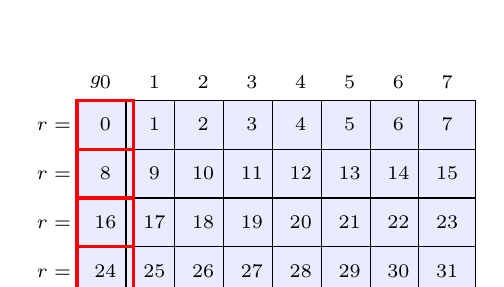
\begin{tikzpicture}[scale=0.62, every node/.style={font=\scriptsize}]
  \node[left] at (-0.15,0) {$r=0$};
  \node[left] at (-0.15,-1) {$r=1$};
  \node[left] at (-0.15,-2) {$r=2$};
  \node[left] at (-0.15,-3) {$r=3$};
  \node[above] at (-0.2,0.55) {$g$};
  \foreach \g in {0,...,7} \node[above] at (\g,0.55) {\g};
  \foreach \r in {0,1,2,3}
    \foreach \g in {0,...,7} {
      \pgfmathtruncatemacro{\s}{8*\r+\g}
      \node[draw, minimum width=7.2mm, minimum height=6.2mm, fill=blue!8] at (\g,-\r) {\s};
    }
  % highlight column group q=0, the four sets B of this tile always hits
  \foreach \r in {0,1,2,3}
    \node[draw, very thick, red, minimum width=7.2mm, minimum height=6.2mm] at (0,-\r) {};
\end{tikzpicture}
\caption{case2 一条 $4$ 行的 $A$ 行带：格子里是组号。红框是列组 $g=0$ 的四个组。$j_0=0$ 的 $B$ 在任何 $k$ 都只碰这四个组。}
\label{fig:c2set}
\end{figure}

列块 $j_0=4q$，$q\in\{0,\ldots,7\}$。$B[k][j_0..j_0+3]$ 的组号是
\begin{equation}
\label{eq:c2b}
\mathrm{set}(B)=8(k\bmod 4)+q.
\end{equation}
它只取四个值：$q,\ 8+q,\ 16+q,\ 24+q$。对照~\eqref{eq:c2set}，这正是 $A$ 行带里列组 $g=q$ 的四条行。别的列组，这条 $B$ 碰不到。$C$ 的四个 store 写的也是这四个组。

\subsection{B 和 C}

$B$：$(32/4)\cdot(32/4)=64$ 个块，每块 $32$ 个 $k$，每个 $k$ 一条 cache 行，
\[
64\cdot32=2048.
\]
也等于 $mnp/(RS)=32768/16$。实测缺失 $2048$，时间命中 $0$，空间命中 $6144$。$2048+6144=8192$，即每条行 $1$ 次缺失、$3$ 次命中。

$C$：$1024/4=256$ 条行。每个块写 $4$ 行 $\times$ $1$ 条行，块与块不共享行（$S=4$ 且对齐）。缺失 $256$，空间命中 $768$，时间命中 $0$。

于是 $A$ 的缺失 $=3200-2048-256=896$。

\subsection{A 的 \texorpdfstring{$896=256+192+448$}{896}}

$A$ 有 $1024/4=256$ 条行，冷缺失 $256$。每个 $i_0$ 有一条行带，$8$ 条行带 $\times$ $32$ 条行 $=256$，全部发生在该行带的第一个列块。

\textbf{每个块恰好 $3$ 次块内重载。}设当前列块是 $q$。由~\eqref{eq:c2b}，$k=4q+t$（$t=0,1,2,3$）时 $k\bmod 4=t$，$B$ 挤掉的是第 $t$ 行、列组 $q$ 那一条。这条行在 $t+1$ 时还要用。所以 $t=0,1,2$ 各造成下一次 $k$ 的一次缺失，共 $3$ 次；$t=3$ 挤掉第 $3$ 行时，列组 $q$ 的四个 $k$ 已经结束。$64$ 个块都经过自己的 $q$，模拟器对 $64$ 个块统计到的块内次数都是 $3$，合计 $64\cdot3=192$。

第一个列块 $q=0$、$i_0=0$ 的前四个 $k$ 是：

\begin{center}
\small
\begin{tabular}{@{}rllll@{}}
\toprule
$k$ & 四行 $A$ 的结果 & 这次 $B$ 挤掉的行\\
\midrule
$0$ & 四行都是冷缺失 & 第 $0$ 行（组 $0$）\\
$1$ & 第 $0$ 行块内缺失，其余三行命中 & 第 $1$ 行（组 $8$）\\
$2$ & 第 $1$ 行块内缺失 & 第 $2$ 行（组 $16$）\\
$3$ & 第 $2$ 行块内缺失 & 第 $3$ 行（组 $24$），随后不再使用\\
\bottomrule
\end{tabular}
\end{center}

$k=4$ 起进入列组 $1$，四行又是冷缺失（本行带第一次读到这些行），不再有块内缺失，直到整个块结束。被挤掉的对象在 $k=1$ 时是 $B[0][0]$ 所在的行：上一步 $B$ 占着组 $0$，$A$ 要回来，于是缺失。

\textbf{第一个列块之后，每个块恰好 $8$ 次换块重载。}块 $q$ 的 $B$ 和最后的 $C$ 只碰列组 $q$ 的四个组，碰不到其他列组。因此一块结束时，被毁掉的 $A$ 行只有列组 $q$。下一块是 $q'=q+1$，它要读全部 $8$ 个列组：

\begin{itemize}
  \item 列组 $q$ 在上一块末尾被 $C$ 写掉了。下一块走到 $k=4q$ 时，四行全部缺失。$(i_0,j_0)=(0,4)$ 时这发生在 $k=0$，被替换出去的是上一块的 $C[r][0]$。
  \item 列组 $q'$ 在本块早期的 $B$ 里就被挤掉。$B$ 的组号始终是列组 $q'$ 那四个。还没走到 $k=4q'$，四条行已经不在了。同一例子里这发生在 $k=4$，被替换出去的是本块的 $B[0][4]$ 到 $B[3][4]$。
  \item 另外六个列组，上一块没有碰它们，本块的 $B$ 在走到它们之前也不碰它们，所以命中。$(0,4)$ 这个块在 $k\ge 8$ 之后没有任何 $A$ 缺失。
\end{itemize}

两类各 $4$ 次，共 $8$ 次。模拟器对 $8$ 条行带、每条 $7$ 个后续列块的统计都是 $8$，没有例外。合计
\[
8\cdot7\cdot8=448.
\]
再加上每块都有的 $3$ 次块内重载。第一个列块没有「上一块」，那 $32$ 次是冷缺失而不是换块重载，块内的 $3$ 次照旧。

验算一条行带，再乘 $8$：
\begin{align*}
\text{第一个列块}&=32+3=35,\\
\text{后 }7\text{ 个列块}&=7\cdot(8+3)=77,\\
\text{一条行带}&=35+77=112,\\
8\text{ 条行带}&=896.
\end{align*}
又写成 $256+192+448=896$。$3200=896+2048+256$。

\subsection{和 baseline 比，以及为什么加速比高于 case1}

\begin{center}
\small
\begin{tabular}{@{}lrrrr@{}}
\toprule
 & baseline 访问/缺失 & 实现访问/缺失 & 访问变成 & 缺失变成\\
\midrule
$A$ & $32768/2240$ & $8192/896$ & $1/4$ & $896/2240$\\
$B$ & $32768/32768$ & $8192/2048$ & $1/4$ & $2048/32768$\\
$C$ & $1024/1024$ & $1024/256$ & 不变 & $1/4$\\
$\mc$ & $36032$ & $3200$ &  & \\
$\mreg$ & $66560$ & $17408$ &  & \\
latency & $607040$ & $65408$ &  & $9.2808$ 倍\\
\bottomrule
\end{tabular}
\end{center}

访问次数的比例和 case1 相同，都是 $R=S=4$ 带来的 $1/4$。加速比更高，是因为 baseline 的 $B$ 更大：$32768$ 次全缺失，光这一项就是 $15\cdot32768=491520$，而实现把这 $32768$ 次 load 收成 $8192$ 次、再收成 $2048$ 次缺失。case1 的 baseline $B$ 只有 $4096$ 次，同样的 $1/4$ 再乘「每条行只缺一次」，绝对数字小一些，加速比就低一些。

$j$ 在外时 $\mc$ 从 $3200$ 变成 $4544$（表~\ref{tab:var}）。$B$ 的列带只占~\eqref{eq:c2b} 的四个组，$32$ 行放不进去，所以不该把 $j$ 放到外面去保 $B$。

\subsection{还可以怎么改}

和 case1 一样，若每个列组开始时把四行 $\times$ $4$ 个 \code{int} 先 load 进寄存器，块内那 $192$ 次缺失会变成命中。按这个顺序重放地址，$\mc$ 从 $3200$ 降到 $3008$，刚好少 $192$。latency 变成 $65408-15\cdot192=65408-2880=62528$，加速比 $607040/62528=9.7081\ldots$。寄存器仍是 $16$ 个 $A$ 加 $16$ 个累加器再加 $8$ 个指针和循环变量，等于 $40$，过线。这是 case2 里能指出具体次数、但在 $36$ 个寄存器里做不到的一项。

垫 \code{pad} 个 \code{int} 再错开 $B$ 的起点，最好的是 \code{pad}$=4$，$\mc$ 只从 $3200$ 降到 $3176$，少 $24$ 次。\code{pad}$=1$ 时 $\mc$ 升到 $5888$。组号冲突主要是「一条行带已经占满 $32$ 个组，而 $B$ 的四个组必然和其中四条 $A$ 行重叠」，不是一个全局相位能躲开的。$k$ 分段写回 $C$ 的三档（段长 $4$、$8$、$16$）latency 分别是 $106624$、$83072$、$71296$，都高于 $65408$。

\subsection{写之前可以自己算的等式}

\begin{enumerate}
  \item $32768\cdot1/2+1024=17408$。
  \item $B$：$64\cdot32=2048$。$C$：$1024/4=256$。
  \item 一条行带 $32+3+7\cdot(8+3)=112$，$8\cdot112=896$。
  \item $896+2048+256=3200$，$15\cdot3200+17408=65408$。
  \item $4\times6$ 的盈亏：$2048/15=136.5$，实测多 $1000$ 次缺失，所以不选。
\end{enumerate}

%----------------------------------------------------------------------
\section{case3：\texorpdfstring{$27\times 41\times 27$}{27x41x27}}
\label{sec:c3}

$A$ 是 $27$ 行 $\times$ $41$ 列，$B$ 是 $41$ 行 $\times$ $27$ 列，$C$ 是 $27$ 行 $\times$ $27$ 列。$k$ 循环长 $41$，不切。$C$ 上的分块是 $4\times6$ 的主块，加上宽 $3$ 或高 $3$ 的边缘。

\subsection{边缘为什么是 \texorpdfstring{$3$}{3}，四块怎么铺}
\label{sec:c3tile}

$27=6\cdot4+3=4\cdot6+3$。行方向主步长 $4$，列方向主步长 $6$，两边余数都是 $3$。主循环的条件是 \code{i0 + 3 < m} 和 \code{j0 + 5 < p}：

\begin{itemize}
  \item \code{i0} 取 $0,4,8,12,16,20$。$20+3=23<27$，$24+3=27$ 不小于 $27$，所以满高的行是 $0$--$23$，共 $6$ 条、每条 $4$ 行。
  \item \code{j0} 取 $0,6,12,18$。$18+5=23<27$，$24+5=29$ 不小于 $27$，满宽的列是 $0$--$23$，共 $4$ 条、每条 $6$ 列。
  \item 列边缘从 \code{j0 = p - 3 = 24} 起，条件 \code{j0 + 2 < p} 只成立这一次，覆盖列 $24,25,26$。
  \item 行边缘从 \code{i0 = m - 3 = 24} 起，同样只走一次，覆盖行 $24,25,26$。
\end{itemize}

四类块互不重叠，并起来是整个 $27\times27$ 的 $C$：

\begin{center}
\begin{tabular}{@{}lrrl@{}}
\toprule
区域 & 块的形状 & 块数 & 覆盖的 $C$\\
\midrule
主块 & $4\times6$ & $6\cdot4=24$ & 行 $0$--$23$，列 $0$--$23$\\
右侧 & $4\times3$ & $6\cdot1=6$ & 行 $0$--$23$，列 $24$--$26$\\
下方 & $3\times6$ & $1\cdot4=4$ & 行 $24$--$26$，列 $0$--$23$\\
右下 & $3\times3$ & $1$ & 行 $24$--$26$，列 $24$--$26$\\
\bottomrule
\end{tabular}
\end{center}

\begin{figure}[ht]
\centering
\begin{tikzpicture}[scale=0.20,font=\footnotesize]
  \foreach \i in {0,4,...,20}
    \foreach \j in {0,6,12,18}
      \draw[fill=green!25] (\j,-\i) rectangle ++(6,-4);
  \foreach \i in {0,4,...,20}
    \draw[fill=orange!35] (24,-\i) rectangle ++(3,-4);
  \foreach \j in {0,6,12,18}
    \draw[fill=blue!18] (\j,-24) rectangle ++(6,-3);
  \draw[fill=red!25] (24,-24) rectangle ++(3,-3);
  \draw[thick] (0,0) rectangle (27,-27);
  \node[above] at (13.5,0.4) {$C$：$27$ 行 $\times$ $27$ 列};
  \node[right,align=left] at (28.2,-6) {$4\times6$，二十四块};
  \node[right,align=left] at (28.2,-12) {$4\times3$，六块};
  \node[right,align=left] at (28.2,-18) {$3\times6$，四块};
  \node[right,align=left] at (28.2,-24) {$3\times3$，一块};
\end{tikzpicture}
\caption{case3 的 $C$。四块区域不重叠。列 $0$--$23$ 与列 $24$--$26$ 的分界、行 $0$--$23$ 与行 $24$--$26$ 的分界都落在元素之间。}
\label{fig:c3}
\end{figure}

$24+3=27$，列和行都盖满，也没有一块被算两次。右侧循环写在每个满高 \code{i0} 的内层、主列循环之后；下方两段写在满高循环之后。这和「\code{i0} 从 $0$ 每次加 $4$、\code{j0} 从 $0$ 每次加 $6$，最后一块用剩余高度和宽度」的地址顺序相同，官方 trace 与按这个规则生成的 $14013$ 个地址逐条一致。

\subsection{寄存器：峰值是 \texorpdfstring{$36$}{36}，不是四段之和}
\label{sec:c3reg}

四段循环前后衔接，前一段的累加器析构之后下一段才声明。\code{printTrace} 的峰值 $36$ 来自主块。探针把四段分开测：

\begin{center}
\begin{tabular}{@{}lrrl@{}}
\toprule
段 & 累加器 & 公式 $R_h S_h+R_h+8$ & 最内层实测\\
\midrule
$4\times6$ & $24$ & $24+4+8=36$ & $36$\\
$4\times3$ & $12$ & $12+4+8=24$ & $24$\\
$3\times6$ & $18$ & $18+3+8=29$ & $29$\\
$3\times3$ & $9$ & $9+3+8=20$ & $20$\\
\bottomrule
\end{tabular}
\end{center}

$36$ 已经顶满。主块里不能再声明任何 \code{reg}，也不能再把 \code{b} 拆成六个。$k$ 结束后主块还剩 $24+6=30$ 个，写回本身不再增加。边缘段更松：$3\times6$ 的 $29$ 仍然小于 $36$，所以写在同一个函数里是合法的。

\subsection{指令数：四段相加，不要用未取整的系数}

一块 $R_h\times S_h$ 的指令数是 $41(R_h+S_h)+R_h S_h$。

\begin{align*}
4\times6&: 41\cdot10+24=434, & 24\cdot434&=10416,\\
4\times3&: 41\cdot7+12=299, & 6\cdot299&=1794,\\
3\times6&: 41\cdot9+18=387, & 4\cdot387&=1548,\\
3\times3&: 41\cdot6+9=255, & 1\cdot255&=255.
\end{align*}
\[
10416+1794=12210,\quad 12210+1548=13758,\quad 13758+255=14013.
\]
用~\eqref{eq:mreg} 复核：$\lceil27/6\rceil=5$，$\lceil27/4\rceil=7$，
\[
\mreg=41\bigl(27\cdot5+27\cdot7\bigr)+729=41\cdot27\cdot12+729=13284+729=14013.
\]
trace 行数是 $14013$。未取整的 $13182.75$ 少算了边缘块把 $A$、$B$ 多 load 的那一部分，不能当理论值。

\[
\mc=5003,\qquad \mathrm{latency}=15\cdot5003+14013=75045+14013=89058.
\]
加速比 $613542/89058=6.889240\ldots$，脚本印成 $6.8892$。

\subsection{为什么主块是 \texorpdfstring{$4\times6$}{4x6}}

$27$ 的正因数是 $1,3,9,27$。同时整除行和列、且 $R(S+1)\le 28$ 的块里，实测最好的是 $1\times27$，latency $154860$；其次 $3\times3$，latency $144630$。两者的指令数就已经高于 $14013$：
\begin{align*}
1\times27&:\ \mreg=27\cdot41\cdot27\Bigl(1+\frac1{27}\Bigr)+729=31725,\\
3\times3&:\ \mreg=29889\cdot\frac23+729=20655.
\end{align*}
$9\times3$ 的寄存器数是 $27+9+8=44$，不合法。所以「为了整除而退回因数」会把 $\mreg$ 抬高几千，cache 上省不回来。

不整除的第二名是 $3\times7$，latency $94125$，比 $89058$ 多 $5067$。$4\times4$ 在 case3 上是 $107307$，比主块多 $18249$。$4\times6$ 把寄存器用满，系数 $1/4+1/6=5/12$ 在合法块里最小；余数只有 $3$，边缘的额外 load（$14013$ 比 $13182.75$ 多出来的那 $830$ 左右）没有把这个优势吃掉。$73$ 个合法块里它是唯一的最小 latency。

$6$ 不整除 $27$，这是已知的。选择它不是因为 $27$ 被 $6$ 整除，而是因为余数小、并且枚举之后 latency 最小。报告里如果只写「$4\times6$ 最优因为 $1/R+1/S$ 最小」，还缺两句：不整除时的 $\mreg$ 要用~\eqref{eq:mreg}，以及第二名的实测 latency 高 $5067$。

\subsection{代码四段}

主块和 case1 的差别只有宽度。累加器是 $4$ 行 $\times$ $6$ 列，\code{c00} 到 \code{c35}。$k$ 循环仍是先 $4$ 个 \code{a}，再把 \code{b} 赋值六次：

\begin{lstlisting}
reg a0 = A[(i0 + 0) * n + k];
reg a1 = A[(i0 + 1) * n + k];
reg a2 = A[(i0 + 2) * n + k];
reg a3 = A[(i0 + 3) * n + k];
reg b = B[k * p + (j0 + 0)];
c00 += a0 * b; c10 += a1 * b; c20 += a2 * b; c30 += a3 * b;
b = B[k * p + (j0 + 1)];
// 同样的四次乘加，列下标换成 1..5
\end{lstlisting}

六个 $B$ 元素仍然沿行连续。它们往往跨两条、有时跨三条 cache 行，不再像 $S=4$ 那样稳定地「$1$ 次缺失加 $3$ 次命中」。先把 $A$ 读进寄存器，至少保证这六个列共用同一批 $A$，不会把 $A$ 的 load 乘上 $6$。

右侧 $4\times3$ 在同一个 \code{i0} 下、主列循环结束之后。累加器换成 $12$ 个，\code{a0}--\code{a3} 仍是四个，因为高度还是 $4$。\code{j0} 固定从 $24$ 出发。下方 $3\times6$ 只有 \code{a0,a1,a2} 和 $18$ 个累加器。右下角 $3\times3$ 是 $9$ 个累加器。四段的 $k$ 都是从 $0$ 到 $40$，不共享累加器：右上角的列和主块的列不重叠，必须各自从 $0$ 累加。

\subsection{B 的 \texorpdfstring{$3024$}{3024} 次缺失}
\label{sec:c3miss}

$B[0][0]$ 的全局下标是 $1107$，$1107\bmod 4=3$。第 $k$ 行、第 $j$ 列在其 cache 行内的偏移是
\[
(1107+27k+j)\bmod 4=(3+3k+j)\bmod 4,
\]
因为 $27\equiv 3\pmod 4$。从偏移 $\mathrm{off}$（$0$ 到 $3$）起连续 $S$ 个 \code{int}，占用的 cache 行数是
\begin{equation}
\label{eq:span}
\lfloor(\mathrm{off}+S-1)/4\rfloor+1.
\end{equation}
$k$ 的余数决定偏移，而且同一个 $k\bmod 4$、同一个 $j_0$，偏移是常数。$k=0..40$ 里，$k\bmod 4=0$ 有 $11$ 个（$0,4,\ldots,40$），其余三个余数各有 $10$ 个。五个列块的行数是：

\begin{center}
\captionof{table}{一个 $i$ 块内，$B$ 切片的 cache 行数。列是 $j_0$，行是 $k\bmod 4$。括号里是偏移。}
\label{tab:blines}
\small
\begin{tabular}{@{}rccccc@{}}
\toprule
$k\bmod 4$ & $j_0=0$（宽 $6$） & $6$ & $12$ & $18$ & $24$（宽 $3$）\\
\midrule
$0$（$11$ 个 $k$） & $3\ (3)$ & $2\ (1)$ & $3\ (3)$ & $2\ (1)$ & $2\ (3)$\\
$1$（$10$ 个） & $2\ (2)$ & $2\ (0)$ & $2\ (2)$ & $2\ (0)$ & $2\ (2)$\\
$2$（$10$ 个） & $2\ (1)$ & $3\ (3)$ & $2\ (1)$ & $3\ (3)$ & $1\ (1)$\\
$3$（$10$ 个） & $2\ (0)$ & $2\ (2)$ & $2\ (0)$ & $2\ (2)$ & $1\ (0)$\\
\bottomrule
\end{tabular}
\end{center}

以左上角为例：偏移 $3$、宽 $6$，$\lfloor(3+5)/4\rfloor+1=3$。把一行乘上 $k$ 的个数再相加：
\begin{align*}
k\bmod 4=0&: 11\cdot(3+2+3+2+2)=11\cdot12=132,\\
k\bmod 4=1&: 10\cdot(2+2+2+2+2)=100,\\
k\bmod 4=2&: 10\cdot(2+3+2+3+1)=110,\\
k\bmod 4=3&: 10\cdot(2+2+2+2+1)=90.
\end{align*}
\[
132+100+110+90=432.
\]
$i$ 方向有 $\lceil27/4\rceil=7$ 个块（$6$ 个高 $4$、$1$ 个高 $3$）。每个 $i$ 块都把全部 $k$、全部列块走一遍，而模拟器记录的 $B$ 时间命中是 $0$，所以每个 $i$ 块都把这 $432$ 条行重新缺失一次：
\[
7\cdot432=3024.
\]
$B$ 的 load 次数是 $41\cdot27\cdot7=7749$。$7749-3024=4725$ 次全是同一切片内部的空间命中。平均每条被碰到的行里有 $7749/3024=41/16=2.5625$ 个本次切片的 \code{int}，命中与缺失之比是 $25/16$，低于 case1、case2 的 $3$。宽 $6$ 从偏移 $3$ 起步时一条行里只剩 $1$ 个 \code{int}，这条行就是一次缺失、零次命中，把平均值拉低。

冷缺失只有 $277$ 次，其余 $3024-277=2747$ 次是冲突重载。$B$ 覆盖的块号从 $276$ 到 $553$，共 $278$ 块；其中块 $553$ 先被 $C$ 碰到，所以算在 $C$ 的冷缺失里，$B$ 的冷缺失是 $278-1=277$。

\subsection{C 的 \texorpdfstring{$282$}{282} 次缺失}

$C$ 的起点下标 $2214\equiv 2\pmod 4$，行宽 $27\equiv 3\pmod 4$。第 $i$ 行起点的行内偏移是 $(2+3i)\bmod 4$。满高的行带从 $i_0=0,4,\ldots,20$ 开始，$4\cdot27=108$ 是 $4$ 的倍数，所以六条满高行带的对齐方式相同。带内四行的起点偏移是
\[
r=0,1,2,3 \quad\text{对应}\quad 2,\ 1,\ 0,\ 3.
\]
宽 $6$ 的切片用~\eqref{eq:span}：偏移 $0$、$1$、$2$ 各占 $2$ 条行，偏移 $3$ 占 $3$ 条行。四行合计 $2+2+2+3=9$，与 $j_0=0,6,12,18$ 无关（列起点每增加 $6\equiv 2\pmod 4$，只是把「占 $3$ 条行」的那一行换到另一行，总和不变）。右侧宽 $3$：四行的行数是 $2,1,1,2$，合计 $6$。

\[
6\text{ 条行带}\cdot(4\cdot9+6)=6\cdot42=252.
\]
下方三行就是上面四行里的前三行，去掉偏移为 $3$ 的那一行。四个宽 $6$ 的块行数是 $6,7,6,7$，和为 $26$；右下角宽 $3$ 是 $2+1+1=4$。下方合计 $30$。
\[
252+30=282.
\]
模拟器：缺失 $282$，空间命中 $447$，时间命中 $0$。$729-282=447$，即每个元素一次 store，每条「块内的 cache 行」缺失一次、行内其余 store 命中。有的 cache 行被相邻两块各写到一部分（宽 $6$ 的边界经常把一条行切开），所以唯一的 $C$ 块只有 $183$ 条（块号 $553$ 到 $735$），缺失次数 $282$ 大于 $183$。多出来的 $282-183=99$ 次是同一条行在另一块里再次缺失。$183$ 次冷缺失说明这 $183$ 条行的第一次访问都算在 $C$ 上，包括和 $B$ 共享的块 $553$：它在第一块主块写 $C[0][0]$ 时被装入，而 $B[40][25]$ 要到列边缘 $j_0=24$ 才读。

三段冷缺失加在一起是全部唯一块：
\[
A\ 的\ 276 + B\ 的\ 277 + C\ 的\ 183 = 736,
\]
与模拟器统计的唯一块数相同。

\subsection{A 的 \texorpdfstring{$1697$}{1697} 次缺失}

$A$ 有 $1107$ 个元素，下标 $0$ 到 $1106$，块号 $0$ 到 $276$，共 $277$ 条行。其中块 $276$ 的第一次访问算在 $B$ 上，所以 $A$ 的冷缺失是 $276$，另外 $1$ 次是 $A$ 第一次读到这块时它已经不在 cache 里，记为「其他」。$276+1=277$，二十七条行都至少缺失过一次。

满高的一条行带是 $4\cdot41=164$ 个 \code{int}。$i_0$ 是 $4$ 的倍数时 $41i_0$ 被 $4$ 整除，行带起点 $16$ 字节对齐，正好 $164/4=41$ 条行。六条满高行带在各自第一个列块上各冷缺失 $41$ 次：$6\cdot41=246$。下方三行是 $3\cdot41=123$ 个 \code{int}，起点同样对齐，占 $\lceil123/4\rceil=31$ 条行，其中一条是块 $276$。实测下方第一个列块冷缺失 $30$，加上那 $1$ 次「其他」，正好 $31$。
\[
246+30+1=277.
\]

其余缺失是重载。按区域加总（每个区域内部，模拟器再按块求和）：

\begin{center}
\captionof{table}{case3 的 $A$ 缺失。$4\times6$ 的块内次数在 $9$ 到 $14$ 之间，不是常数，所以表里只给区域合计。}
\label{tab:c3a}
\small
\begin{tabular}{@{}lrrrrr@{}}
\toprule
区域 & 块数 & 冷 & 换列块 & 块内 & 其他\\
\midrule
$4\times6$ & $24$ & $246$ & $704$ & $272$ & $0$\\
$4\times3$ & $6$ & $0$ & $234$ & $52$ & $0$\\
$3\times6$ & $4$ & $30$ & $87$ & $35$ & $1$\\
$3\times3$ & $1$ & $0$ & $29$ & $7$ & $0$\\
\midrule
合计 & $35$ & $276$ & $1054$ & $366$ & $1$\\
\bottomrule
\end{tabular}
\end{center}

\[
276+1054+366+1=1697.
\]
换行带的次数是 $0$：每一行只属于一个 $i_0$。右侧 $4\times3$ 没有冷缺失，因为它不是该行带的第一个列块。

块内次数不再是 case2 的「每块恰好 $3$」。行宽 $41\equiv 1\pmod 4$，每一行比上一行多错开 $1$ 个 \code{int}，连续四个 $k$ 不一定是一条 cache 行；列宽 $6$ 又不对齐。同一个主块里，块内次数在 $9$ 与 $14$ 之间变化。强行写成一个与 $j_0$ 无关的常数会和表~\ref{tab:c3a} 矛盾。能对上个位的是区域合计，以及下面这一次具体的冲突，用来说明「块内」在 case3 里仍是 $B$ 把刚用过的 $A$ 行挤掉。

第一块主块，$i_0=j_0=0$，$k=0$ 读了 $A[2][0]$。它的下标是 $2\cdot41=82$，块号 $\lfloor82/4\rfloor=20$，组号 $20$。紧接着读 $B[0][0]$，全局下标 $1107$，块号 $276$，组号也是 $20$（$276=8\cdot32+20$）。$B$ 把块 $20$ 挤出。$k=1$ 的 $A[2][1]$ 还在块 $20$ 里，于是块内缺失，被替换出去的正是 $B[0][0]$ 所在的那一条行。这一块主块一共 $52$ 次 $A$ 缺失，其中冷缺失 $41$、重载 $11$。$52$ 已经多于 case2 一个块的 $3$ 次块内缺失，因为一条行带有 $41$ 条行，大于 $32$ 个组，行带自己就放不进 cache。

这也是 case3 的 $A$ 缺失比例更高的原因。case2 一条行带 $32$ 条行，刚好铺满，换列块时只有 $8$ 条要重读。case3 一条满高行带 $41$ 条行，第一个列块之后的每个列块都要重读大约 $40$ 条（表里 $4\times6$ 的换块合计 $704$，而满高行带的后续列块有 $6\cdot3=18$ 个，$704$ 里还包括右侧块；$18$ 个后续主块若各约 $39$ 次，就在 $700$ 上下）。行带大于 cache，换块重载接近「整条行带再读一遍」。

\subsection{和 baseline 比}

\begin{center}
\small
\begin{tabular}{@{}lrrrr@{}}
\toprule
 & baseline 访问/缺失 & 实现访问/缺失\\
\midrule
$A$ & $29889/6284$ & $5535/1697$\\
$B$ & $29889/29889$ & $7749/3024$\\
$C$ & $729/696$ & $729/282$\\
$\mc$ & $36869$ & $5003$\\
$\mreg$ & $60507$ & $14013$\\
latency & $613542$ & $89058$\\
\bottomrule
\end{tabular}
\end{center}

$A$ 的访问次数 $5535=27\cdot41\cdot5$，即每个 $A$ 元素 load $\lceil27/6\rceil=5$ 次，而不是整除公式里的 $27/6=4.5$ 次。$B$ 的访问次数 $7749=41\cdot27\cdot7$，每个 $B$ 元素 load $7$ 次。baseline 的 $B$ 仍然是 $29889$ 次全缺失。实现把它收成 $7749$ 次 load、$3024$ 次缺失。$C$ 的 store 次数不变，缺失从 $696$ 降到 $282$，因为一个块内的连续列会把同一条行的若干个 \code{int} 一次写完。

加速比 $6.8892$ 低于 case1、case2。行宽 $41$、列宽 $27$ 都不是 $4$ 的倍数，$S$ 也不能取 $4$ 同时保持 $1/R+1/S$ 最小，B、C 的「每 $4$ 个 \code{int} 只缺 $1$ 次」不再成立。权重却是 $0.4$。三个加速比的精确加权是 $8.0131$，只比满分线 $8$ 高 $0.0131$。case3 的权重是 $0.4$，大约再低 $0.033$ 的加速比，$W$ 就会落到 $8$ 上。余量不大，这个 case 的边缘和行数手算值得在报告里留位置。

\subsection{还可以怎么改}

表~\ref{tab:var}：$j$ 在外，$\mc$ 从 $5003$ 变成 $5055$；先 $B$ 后 $A$，变成 $5002$，latency $89043$，四位小数的加速比看起来几乎不动。$k$ 段长 $4$、$8$、$16$ 的 latency 是 $122958$、$109218$、$99504$，都高于 $89058$。

垫偏移的反事实布局里，最好的 \code{pad}$=77$，$\mc$ 从 $5003$ 降到 $4975$，少 $28$ 次。\code{buffer} 只有 $64$ 个 \code{int}，一条满高 $A$ 行带是 $4\cdot41=164$ 个 \code{int}，放不下。少 $28$ 次缺失值 $15\cdot28=420$ 的 latency，相对 $89058$ 不到百分之一。

case2 那种「把一整条 $A$ 行提前放进寄存器」在这里更紧：行宽 $41$，连续四个 $k$ 常常不是一条对齐的 cache 行，而主块已经用满 $36$ 个寄存器，连多留一个 \code{b} 都不行。

\subsection{写之前可以自己算的等式}

\begin{enumerate}
  \item $24\cdot434+6\cdot299+4\cdot387+255=14013$。
  \item $4\cdot6+4+8=36$，$3\cdot6+3+8=29$。
  \item $B$：$132+100+110+90=432$，$7\cdot432=3024$。
  \item $C$：$6\cdot42+26+4=282$。
  \item $A$：$246+30+1=277$ 条行，$276+1054+366+1=1697$。
  \item $1697+3024+282=5003$，$15\cdot5003+14013=89058$。
\end{enumerate}

%----------------------------------------------------------------------
\section{三个 case 合在一起}
\label{sec:together}

\begin{center}
\captionof{table}{实现与 baseline。加速比保留评测脚本的四位小数；加权用的是未舍入的比值。}
\label{tab:all}
\small
\setlength{\tabcolsep}{4pt}
\begin{tabular}{@{}lrrrrrr@{}}
\toprule
case & 块形 & 寄存器 & $\mc$ & $\mreg$ & latency & 加速比\\
\midrule
case0 & 不优化 & $10$ & $3$ & $20$ & $65$ & $1.0000$\\
case1 & $4\times4$ & $28$ & $496$ & $2304$ & $9744$ & $8.2438$\\
case2 & $4\times4$ & $28$ & $3200$ & $17408$ & $65408$ & $9.2808$\\
case3 & $4\times6$ 加边缘 & $36$ & $5003$ & $14013$ & $89058$ & $6.8892$\\
\midrule
\multicolumn{6}{r}{加权 $W$} & $8.0131$\\
\bottomrule
\end{tabular}
\end{center}

case0 的 $2\times2\times2$ 只有三条 cache 行（$A$、$B$、$C$ 各 $4$ 个 \code{int}，各一条），缺失 $3$，指令数 $2\cdot2\cdot(4+1)=20$，latency $65$。实现和 baseline 相同，加速比 $1$，权重 $0$。

三个计分 case 的共同结构是：寄存器里留住一个 $R\times S$ 的 $C$ 小块，$k$ 一次走完；每个 $k$ 只 load $R$ 个 $A$ 和 $S$ 个 $B$，而且 $B$ 沿行连续读。分叉只在块形。case1 与 case2 选择 $4\times4$，是因为在对齐的 $16$ 和 $32$ 上，它的 latency 是合法块里最小的（case1 与 $5\times4$ 并列，用整除和寄存器个数打破）。case3 选择 $4\times6$，是因为 $27$ 的因数块指令数太高，而 $4\times6$ 在 $73$ 个合法块的实测里 latency 最小；余数 $3$ 用三套更小的累加器补上，峰值仍由主块的 $36$ 决定。

若按「加速比高、并且缺失规律能写成对每一个块都成立的等式」来看，case2 最整齐：$64$ 个块的块内次数都是 $3$，后续列块的换块次数都是 $8$。case1 是同一套组冲突，但四行只占半个 cache，所以表~\ref{tab:c1tiles} 里出现 $0$ 和 $3$、$4$ 和 $8$ 的交替。case3 的 B、C 仍能手算到个位，$A$ 的块内次数随对齐变化，只能分区域合计。模板要求你自己排「最优秀的实现」。上面这三条是排序时可以用的事实，不是排好的名单。

%----------------------------------------------------------------------
\section{写报告时可以怎么组织}
\label{sec:write}

模板的字数是报告的约束，不是手册的约束。下面只给结构和该出现的事实。句子要你自己写。不要把本节扩写成带「综上所述」「显著提升」的段落再交上去；模板明确不希望用空话填字数。

\subsection{亮点}

建议四条，按对 latency 的影响从大到小。每条用一个词起头，后面一句说清它减少的是 $\mreg$ 还是 $\mc$：

\begin{enumerate}
  \item 寄存器分块。点明 $RS$ 个累加器、$k$ 走完再写，$A$ 每个元素 load $p/S$ 或 $\lceil p/S\rceil$ 次而不是 $p$ 次。可以带~\eqref{eq:mreg-div} 或~\eqref{eq:mreg}，二选一，case3 必须是带向上取整的那一个。
  \item 块形是按 latency 选的，不是按 $1/R+1/S$ 最小选的。点一个被淘汰的对照：case1/2 的 $4\times6$（指令更少、latency 更高，写出 $\Delta_r/15$ 和实际多出来的缺失），case3 的某个整除块（$3\times3$ 或 $1\times27$ 的 latency）。
  \item $B$ 沿行读，使对齐时一条 cache 行提供 $3$ 次命中。case3 要改口：宽 $6$ 经常跨 $2$ 到 $3$ 条行，所以命中比不是 $3$，但仍然比 baseline 的列访问（命中 $0$）好。给出 $3024$ 这个手算结果。
  \item 只在 case3 写边缘：$27=24+3$，四类块的个数 $24,6,4,1$，寄存器峰值 $36$ 而不是四段相加。
\end{enumerate}

如果还想加第五条，只能加你确实依赖的实测，例如「$j$ 在外使 case2 的 $\mc$ 从 $3200$ 变成 $4544$，所以 $i$ 在外」。不要把没有实现的 $k$ 分段写成已经使用的优化。

\subsection{三个 case 的排序}

模板有一小节要求把你认为最好的实现排在前面。可以用的尺度有三条，它们不一定给出同一个第一名，你要选一个并说你用的是哪一个：

\begin{itemize}
  \item 加速比：$9.2808 > 8.2438 > 6.8892$，即 case2、case1、case3。
  \item 缺失能否写成对每个块都成立的等式：case2 可以（块内 $3$、换块 $8$），case1 要一张 $16$ 行的表，case3 的 $A$ 只能分区域合计。
  \item 离满分线的贡献：case3 权重 $0.4$，而 $W$ 只比 $8$ 高 $0.0131$。若你认为「把最容易掉下满分线的 case 写清楚」也是一种好坏，case3 会靠前。这是写作上的判断，不是性能上的判断。
\end{itemize}

\subsection{每个 case 的四段}

每个 case 建议四段，段内用手册里已经算平的等式，不要再引入新的未测数字。

\begin{enumerate}
  \item \textbf{结果。}块形、寄存器峰值、$\mc$、$\mreg$、latency、加速比。case3 加上四类块的个数。
  \item \textbf{为什么是这个块形。}写出约束 $RS+R+8\le 36$。然后只留一个对照：它的 $\mreg$、$\mc$、latency，以及盈亏平衡 $\Delta_r/15$ 是否被打破。case1 若提到 $5\times4$，要说明两者 latency 相同，选择来自整除和 $28<33$。
  \item \textbf{缺失。}先写 $\mreg$ 的代入。再写 $B$ 和 $C$ 的行数（case1：$256$ 和 $64$；case2：$2048$ 和 $256$；case3：$7\cdot432=3024$ 和 $252+30=282$）。最后写 $A$：case2 用 $256+192+448$，并说明 $3$ 和 $8$ 从哪两个组号公式来；case1 说明 $64+24+88$，并指出低半区和高半区不一样；case3 用表~\ref{tab:c3a} 的合计，并说明块内次数不是常数，所以不假装有一个与 case2 相同的 $3$。
  \item \textbf{相对 baseline。}各用一行对比 $B$：baseline 命中次数是 $0$，实现是「每条行缺失一次、行内其余命中」。$C$ 的访问次数不变、缺失下降，因为写回从「每个 $j$ 隔着整个 $k$ 循环」变成「一个块的连续列一次写完」。
\end{enumerate}

case 与 case 之间相同的寄存器计数不要写三遍。模板允许你改报告结构。可以把第~\ref{sec:formula}~节的公式放在三个 case 之前，每个 case 只做代入。

代码每次只贴一个循环或一次 $k$ 迭代，后面跟一句它对应的访存次数。不要把 $16$ 个累加器的声明和 $16$ 个 store 都贴全；写「$4$ 行 $\times$ $4$ 列，共 $16$ 个，结构相同」即可。

若你把枚举表放进报告，写上复现命令 \code{python3 manual/scripts/analyze\_partb.py}，并说明访存顺序与 \code{gemm\_case1} 相同、$4\times4$、$4\times6$、$5\times4$、$3\times7$ 等行用 \code{csim-ref} 对过。完整表太长就只留每个 case 的前几名，其余放在你自己的附录或直接不放。知是平台仍然只交三个文件，超长表格要事先问过助教才作为附加材料。

\subsection{不要写进 case 正文的内容}

\begin{itemize}
  \item cache 组相联、LRU 的一般定义。$E=1$，报告里一句「直接映射、$32$ 组、块 $16$ 字节」就够。
  \item 没有实测的改进。$k$ 分段、垫 \code{pad}、把整条 $A$ 行放进寄存器，这些手册里是「测过但没有采用」或「寄存器不够」。若你想体现思考，放在反馈或 case 最后，用本节表格里的 latency 说明为什么不采用，不要写成已经实现的优化。
  \item 三个 case 各贴一份几乎相同的 $4\times4$ 代码。case2 写「与 case1 相同，只换维度」，把篇幅留给组号~\eqref{eq:c2set} 和~\eqref{eq:c2b}。
\end{itemize}

\subsection{反馈和参考资料}

模板的反馈节、参考资料节不是这三个 case 的分析。手册不准备这两节的句子。若报告里用到了块形枚举或本手册的分类，参考资料里应能让助教找到实验 README（代价模型、$W$ 的定义）、\code{demo.cpp}（什么算一条访存、什么占寄存器），以及你实际跑过的脚本路径。CS:APP 的 blocking 材料可以作为「为什么分块」的外部来源，但它不包含本实验 $36$ 个寄存器和 $15:1$ 的具体数字，数字仍要来自你自己的评测。
)


\appendix
\section{全部合法块形}
\label{sec:sweep}

三张表由 \code{manual/scripts/analyze\_partb.py} 生成，顺序是 latency 从小到大。访存顺序与第~\ref{sec:formula}~节的伪代码相同。加速比的分母是该 case 的 baseline latency。星号和 \code{csim-ref} 复核见第~\ref{sec:choose}~节，本表其余行使用同一个、已与官方 trace 对齐过的模拟器。

\begingroup
\footnotesize
\setlength{\tabcolsep}{3pt}
\setlength{\LTcapwidth}{\textwidth}
\setlength{\LTleft}{0pt plus 1fill}
\setlength{\LTright}{0pt plus 1fill}
% auto-generated by analyze_partb.py — do not edit
\begin{longtable}{@{}rrrrrrrrrrr@{}}
\caption{case1（$16\times 16\times 16$）全部满足 $RS+R+8\le 36$ 的 $R\times S$，按 latency 从小到大。加粗行是实现采用的块形。「整除」表示 $R\mid 16$ 且 $S\mid 16$。A、B、C 三列是各自的 cache 缺失次数。}
\label{tab:sweep-case1}\\
\toprule $R$ & $S$ & 寄存器 & 整除 & $miss_{reg}$ & $miss_{cache}$ & A & B & C & latency & 加速比\\\midrule\endfirsthead
\toprule $R$ & $S$ & 寄存器 & 整除 & $miss_{reg}$ & $miss_{cache}$ & A & B & C & latency & 加速比\\\midrule\endhead
\bottomrule\endfoot
\textbf{4} & \textbf{4} & 28 & \textbf{是} & 2304 & 496 & 176 & 256 & 64 & 9744 & 8.2438\\
5 & 4 & 33 & 否 & 2304 & 496 & 176 & 256 & 64 & 9744 & 8.2438\\
4 & 6 & 36 & 否 & 2048 & 590 & 190 & 320 & 80 & 10898 & 7.3709\\
3 & 8 & 35 & 否 & 2304 & 600 & 152 & 384 & 64 & 11304 & 7.1062\\
3 & 4 & 23 & 否 & 2816 & 624 & 176 & 384 & 64 & 12176 & 6.5972\\
8 & 2 & 32 & 是 & 2816 & 648 & 264 & 256 & 128 & 12536 & 6.4078\\
2 & 8 & 26 & 是 & 2816 & 728 & 152 & 512 & 64 & 13736 & 5.8480\\
2 & 12 & 34 & 否 & 2816 & 728 & 152 & 512 & 64 & 13736 & 5.8480\\
3 & 6 & 29 & 否 & 2560 & 750 & 190 & 480 & 80 & 13810 & 5.8167\\
6 & 3 & 32 & 否 & 2560 & 776 & 264 & 384 & 128 & 14200 & 5.6569\\
7 & 3 & 36 & 否 & 2560 & 776 & 264 & 384 & 128 & 14200 & 5.6569\\
4 & 5 & 32 & 否 & 2304 & 794 & 234 & 448 & 112 & 14214 & 5.6513\\
2 & 4 & 18 & 是 & 3328 & 752 & 176 & 512 & 64 & 14608 & 5.4989\\
6 & 2 & 26 & 否 & 3072 & 776 & 264 & 384 & 128 & 14712 & 5.4600\\
7 & 2 & 29 & 否 & 3072 & 776 & 264 & 384 & 128 & 14712 & 5.4600\\
3 & 7 & 32 & 否 & 2560 & 884 & 212 & 576 & 96 & 15820 & 5.0776\\
9 & 2 & 35 & 否 & 2816 & 868 & 484 & 256 & 128 & 15836 & 5.0725\\
2 & 9 & 28 & 否 & 2816 & 878 & 158 & 640 & 80 & 15986 & 5.0249\\
2 & 10 & 30 & 否 & 2816 & 878 & 158 & 640 & 80 & 15986 & 5.0249\\
2 & 11 & 32 & 否 & 2816 & 878 & 158 & 640 & 80 & 15986 & 5.0249\\
2 & 13 & 36 & 否 & 2816 & 878 & 158 & 640 & 80 & 15986 & 5.0249\\
4 & 3 & 24 & 否 & 2816 & 904 & 264 & 512 & 128 & 16376 & 4.9052\\
5 & 3 & 28 & 否 & 2816 & 904 & 264 & 512 & 128 & 16376 & 4.9052\\
2 & 6 & 22 & 否 & 3072 & 910 & 190 & 640 & 80 & 16722 & 4.8037\\
4 & 2 & 20 & 是 & 3328 & 904 & 264 & 512 & 128 & 16888 & 4.7565\\
5 & 2 & 23 & 否 & 3328 & 904 & 264 & 512 & 128 & 16888 & 4.7565\\
3 & 5 & 26 & 否 & 2816 & 1018 & 234 & 672 & 112 & 18086 & 4.4414\\
2 & 7 & 24 & 否 & 3072 & 1076 & 212 & 768 & 96 & 19212 & 4.1811\\
3 & 3 & 20 & 否 & 3328 & 1160 & 264 & 768 & 128 & 20728 & 3.8753\\
3 & 2 & 17 & 否 & 3840 & 1160 & 264 & 768 & 128 & 21240 & 3.7819\\
2 & 5 & 20 & 否 & 3328 & 1242 & 234 & 896 & 112 & 21958 & 3.6583\\
1 & 16 & 25 & 是 & 4608 & 1176 & 88 & 1024 & 64 & 22248 & 3.6106\\
8 & 1 & 24 & 是 & 4864 & 1208 & 440 & 512 & 256 & 22984 & 3.4950\\
1 & 8 & 17 & 是 & 4864 & 1240 & 152 & 1024 & 64 & 23464 & 3.4235\\
1 & 12 & 21 & 否 & 4864 & 1240 & 152 & 1024 & 64 & 23464 & 3.4235\\
1 & 4 & 13 & 是 & 5376 & 1264 & 176 & 1024 & 64 & 24336 & 3.3008\\
2 & 3 & 16 & 否 & 3840 & 1416 & 264 & 1024 & 128 & 25080 & 3.2029\\
2 & 2 & 14 & 是 & 4352 & 1416 & 264 & 1024 & 128 & 25592 & 3.1388\\
6 & 1 & 20 & 否 & 5120 & 1464 & 440 & 768 & 256 & 27080 & 2.9663\\
7 & 1 & 22 & 否 & 5120 & 1464 & 440 & 768 & 256 & 27080 & 2.9663\\
1 & 9 & 18 & 否 & 4864 & 1518 & 158 & 1280 & 80 & 27634 & 2.9069\\
1 & 10 & 19 & 否 & 4864 & 1518 & 158 & 1280 & 80 & 27634 & 2.9069\\
1 & 11 & 20 & 否 & 4864 & 1518 & 158 & 1280 & 80 & 27634 & 2.9069\\
1 & 13 & 22 & 否 & 4864 & 1518 & 158 & 1280 & 80 & 27634 & 2.9069\\
1 & 14 & 23 & 否 & 4864 & 1518 & 158 & 1280 & 80 & 27634 & 2.9069\\
1 & 15 & 24 & 否 & 4864 & 1518 & 158 & 1280 & 80 & 27634 & 2.9069\\
1 & 6 & 15 & 否 & 5120 & 1550 & 190 & 1280 & 80 & 28370 & 2.8314\\
9 & 1 & 26 & 否 & 4864 & 1660 & 892 & 512 & 256 & 29764 & 2.6988\\
4 & 1 & 16 & 是 & 5376 & 1720 & 440 & 1024 & 256 & 31176 & 2.5766\\
5 & 1 & 18 & 否 & 5376 & 1720 & 440 & 1024 & 256 & 31176 & 2.5766\\
1 & 7 & 16 & 否 & 5120 & 1844 & 212 & 1536 & 96 & 32780 & 2.4505\\
10 & 1 & 28 & 否 & 4864 & 2112 & 1344 & 512 & 256 & 36544 & 2.1981\\
1 & 5 & 14 & 否 & 5376 & 2138 & 234 & 1792 & 112 & 37446 & 2.1452\\
3 & 1 & 14 & 否 & 5888 & 2232 & 440 & 1536 & 256 & 39368 & 2.0404\\
1 & 3 & 12 & 否 & 5888 & 2440 & 264 & 2048 & 128 & 42488 & 1.8906\\
1 & 2 & 11 & 是 & 6400 & 2440 & 264 & 2048 & 128 & 43000 & 1.8681\\
11 & 1 & 30 & 否 & 4864 & 2564 & 1796 & 512 & 256 & 43324 & 1.8541\\
2 & 1 & 12 & 是 & 6400 & 2744 & 440 & 2048 & 256 & 47560 & 1.6890\\
12 & 1 & 32 & 否 & 4864 & 3032 & 2264 & 512 & 256 & 50344 & 1.5956\\
13 & 1 & 34 & 否 & 4864 & 3486 & 2718 & 512 & 256 & 57154 & 1.4055\\
14 & 1 & 36 & 否 & 4864 & 3940 & 3172 & 512 & 256 & 63964 & 1.2558\\
1 & 1 & 10 & 是 & 8448 & 4792 & 440 & 4096 & 256 & 80328 & 1.0000\\
\end{longtable}

% auto-generated by analyze_partb.py — do not edit
\begin{longtable}{@{}rrrrrrrrrrr@{}}
\caption{case2（$32\times 32\times 32$）全部满足 $RS+R+8\le 36$ 的 $R\times S$，按 latency 从小到大。加粗行是实现采用的块形。「整除」表示 $R\mid 32$ 且 $S\mid 32$。A、B、C 三列是各自的 cache 缺失次数。}
\label{tab:sweep-case2}\\
\toprule $R$ & $S$ & 寄存器 & 整除 & $miss_{reg}$ & $miss_{cache}$ & A & B & C & latency & 加速比\\\midrule\endfirsthead
\toprule $R$ & $S$ & 寄存器 & 整除 & $miss_{reg}$ & $miss_{cache}$ & A & B & C & latency & 加速比\\\midrule\endhead
\bottomrule\endfoot
\textbf{4} & \textbf{4} & 28 & \textbf{是} & 17408 & 3200 & 896 & 2048 & 256 & 65408 & 9.2808\\
3 & 8 & 35 & 否 & 16384 & 3904 & 832 & 2816 & 256 & 74944 & 8.0999\\
4 & 6 & 36 & 否 & 15360 & 4200 & 1032 & 2816 & 352 & 78360 & 7.7468\\
3 & 4 & 23 & 否 & 20480 & 3968 & 896 & 2816 & 256 & 80000 & 7.5880\\
4 & 5 & 32 & 否 & 16384 & 4888 & 1144 & 3328 & 416 & 89704 & 6.7671\\
3 & 7 & 32 & 否 & 17408 & 5256 & 1032 & 3872 & 352 & 96248 & 6.3070\\
3 & 6 & 29 & 否 & 18432 & 5256 & 1032 & 3872 & 352 & 97272 & 6.2406\\
2 & 12 & 34 & 否 & 20480 & 5152 & 800 & 4096 & 256 & 97760 & 6.2095\\
2 & 8 & 26 & 是 & 21504 & 5184 & 832 & 4096 & 256 & 99264 & 6.1154\\
5 & 4 & 33 & 否 & 16384 & 5672 & 3624 & 1792 & 256 & 101464 & 5.9828\\
2 & 4 & 18 & 是 & 25600 & 5248 & 896 & 4096 & 256 & 104320 & 5.8190\\
4 & 3 & 24 & 否 & 20480 & 5952 & 1344 & 4096 & 512 & 109760 & 5.5306\\
3 & 5 & 26 & 否 & 19456 & 6136 & 1144 & 4576 & 416 & 111496 & 5.4445\\
4 & 2 & 20 & 是 & 25600 & 5952 & 1344 & 4096 & 512 & 114880 & 5.2841\\
2 & 11 & 32 & 否 & 20480 & 6320 & 880 & 5120 & 320 & 115280 & 5.2658\\
2 & 13 & 36 & 否 & 20480 & 6320 & 880 & 5120 & 320 & 115280 & 5.2658\\
2 & 10 & 30 & 否 & 21504 & 6384 & 944 & 5120 & 320 & 117264 & 5.1767\\
2 & 9 & 28 & 否 & 21504 & 6952 & 968 & 5632 & 352 & 125784 & 4.8261\\
2 & 7 & 24 & 否 & 22528 & 7016 & 1032 & 5632 & 352 & 127768 & 4.7511\\
2 & 6 & 22 & 否 & 23552 & 7016 & 1032 & 5632 & 352 & 128792 & 4.7133\\
3 & 3 & 20 & 否 & 23552 & 7488 & 1344 & 5632 & 512 & 135872 & 4.4677\\
3 & 2 & 17 & 否 & 28672 & 7488 & 1344 & 5632 & 512 & 140992 & 4.3055\\
2 & 5 & 20 & 否 & 24576 & 8216 & 1144 & 6656 & 416 & 147816 & 4.1067\\
5 & 3 & 28 & 否 & 19456 & 9144 & 5048 & 3584 & 512 & 156616 & 3.8760\\
1 & 16 & 25 & 是 & 35840 & 9152 & 704 & 8192 & 256 & 173120 & 3.5065\\
1 & 20 & 29 & 否 & 35840 & 9152 & 704 & 8192 & 256 & 173120 & 3.5065\\
1 & 24 & 33 & 否 & 35840 & 9152 & 704 & 8192 & 256 & 173120 & 3.5065\\
1 & 12 & 21 & 否 & 36864 & 9248 & 800 & 8192 & 256 & 175584 & 3.4573\\
1 & 8 & 17 & 是 & 37888 & 9280 & 832 & 8192 & 256 & 177088 & 3.4279\\
2 & 3 & 16 & 否 & 28672 & 10048 & 1344 & 8192 & 512 & 179392 & 3.3839\\
1 & 4 & 13 & 是 & 41984 & 9344 & 896 & 8192 & 256 & 182144 & 3.3327\\
2 & 2 & 14 & 是 & 33792 & 10048 & 1344 & 8192 & 512 & 184512 & 3.2900\\
6 & 3 & 32 & 否 & 18432 & 11112 & 7528 & 3072 & 512 & 185112 & 3.2793\\
1 & 17 & 26 & 否 & 35840 & 10232 & 728 & 9216 & 288 & 189320 & 3.2064\\
1 & 18 & 27 & 否 & 35840 & 10232 & 728 & 9216 & 288 & 189320 & 3.2064\\
1 & 19 & 28 & 否 & 35840 & 10232 & 728 & 9216 & 288 & 189320 & 3.2064\\
1 & 21 & 30 & 否 & 35840 & 10232 & 728 & 9216 & 288 & 189320 & 3.2064\\
1 & 22 & 31 & 否 & 35840 & 10232 & 728 & 9216 & 288 & 189320 & 3.2064\\
1 & 23 & 32 & 否 & 35840 & 10232 & 728 & 9216 & 288 & 189320 & 3.2064\\
1 & 25 & 34 & 否 & 35840 & 10232 & 728 & 9216 & 288 & 189320 & 3.2064\\
1 & 26 & 35 & 否 & 35840 & 10232 & 728 & 9216 & 288 & 189320 & 3.2064\\
1 & 27 & 36 & 否 & 35840 & 10232 & 728 & 9216 & 288 & 189320 & 3.2064\\
5 & 2 & 23 & 否 & 24576 & 11064 & 6968 & 3584 & 512 & 190536 & 3.1860\\
1 & 14 & 23 & 否 & 36864 & 10360 & 856 & 9216 & 288 & 192264 & 3.1573\\
7 & 3 & 36 & 否 & 17408 & 11856 & 8784 & 2560 & 512 & 195248 & 3.1091\\
1 & 11 & 20 & 否 & 36864 & 11440 & 880 & 10240 & 320 & 208464 & 2.9120\\
1 & 13 & 22 & 否 & 36864 & 11440 & 880 & 10240 & 320 & 208464 & 2.9120\\
1 & 15 & 24 & 否 & 36864 & 11472 & 912 & 10240 & 320 & 208944 & 2.9053\\
1 & 10 & 19 & 否 & 37888 & 11504 & 944 & 10240 & 320 & 210448 & 2.8845\\
4 & 1 & 16 & 是 & 41984 & 11456 & 2240 & 8192 & 1024 & 213824 & 2.8390\\
1 & 9 & 18 & 否 & 37888 & 12584 & 968 & 11264 & 352 & 226648 & 2.6783\\
1 & 7 & 16 & 否 & 38912 & 12648 & 1032 & 11264 & 352 & 228632 & 2.6551\\
1 & 6 & 15 & 否 & 39936 & 12648 & 1032 & 11264 & 352 & 229656 & 2.6433\\
6 & 2 & 26 & 否 & 23552 & 14312 & 10728 & 3072 & 512 & 238232 & 2.5481\\
7 & 2 & 29 & 否 & 22528 & 15696 & 12624 & 2560 & 512 & 257968 & 2.3532\\
3 & 1 & 14 & 否 & 45056 & 14528 & 2240 & 11264 & 1024 & 262976 & 2.3083\\
1 & 5 & 14 & 否 & 40960 & 14872 & 1144 & 13312 & 416 & 264040 & 2.2990\\
9 & 2 & 35 & 否 & 21504 & 17546 & 14986 & 2048 & 512 & 284694 & 2.1323\\
8 & 2 & 32 & 是 & 21504 & 18944 & 16384 & 2048 & 512 & 305664 & 1.9860\\
1 & 3 & 12 & 否 & 45056 & 18240 & 1344 & 16384 & 512 & 318656 & 1.9050\\
1 & 2 & 11 & 是 & 50176 & 18240 & 1344 & 16384 & 512 & 323776 & 1.8749\\
2 & 1 & 12 & 是 & 50176 & 19648 & 2240 & 16384 & 1024 & 344896 & 1.7601\\
5 & 1 & 18 & 否 & 40960 & 21848 & 13656 & 7168 & 1024 & 368680 & 1.6465\\
6 & 1 & 20 & 否 & 39936 & 28456 & 21288 & 6144 & 1024 & 466776 & 1.3005\\
7 & 1 & 22 & 否 & 38912 & 31280 & 25136 & 5120 & 1024 & 508112 & 1.1947\\
14 & 1 & 36 & 否 & 36864 & 33048 & 28952 & 3072 & 1024 & 532584 & 1.1398\\
13 & 1 & 34 & 否 & 36864 & 34972 & 30876 & 3072 & 1024 & 561444 & 1.0812\\
9 & 1 & 26 & 否 & 37888 & 35050 & 29930 & 4096 & 1024 & 563638 & 1.0770\\
10 & 1 & 28 & 否 & 37888 & 35964 & 30844 & 4096 & 1024 & 577348 & 1.0514\\
11 & 1 & 30 & 否 & 36864 & 36864 & 32768 & 3072 & 1024 & 589824 & 1.0292\\
12 & 1 & 32 & 否 & 36864 & 36864 & 32768 & 3072 & 1024 & 589824 & 1.0292\\
8 & 1 & 24 & 是 & 37888 & 37888 & 32768 & 4096 & 1024 & 606208 & 1.0014\\
1 & 1 & 10 & 是 & 66560 & 36032 & 2240 & 32768 & 1024 & 607040 & 1.0000\\
\end{longtable}

% auto-generated by analyze_partb.py — do not edit
\begin{longtable}{@{}rrrrrrrrrrr@{}}
\caption{case3（$27\times 41\times 27$）全部满足 $RS+R+8\le 36$ 的 $R\times S$，按 latency 从小到大。加粗行是实现采用的块形。「整除」表示 $R\mid 27$ 且 $S\mid 27$。A、B、C 三列是各自的 cache 缺失次数。}
\label{tab:sweep-case3}\\
\toprule $R$ & $S$ & 寄存器 & 整除 & $miss_{reg}$ & $miss_{cache}$ & A & B & C & latency & 加速比\\\midrule\endfirsthead
\toprule $R$ & $S$ & 寄存器 & 整除 & $miss_{reg}$ & $miss_{cache}$ & A & B & C & latency & 加速比\\\midrule\endhead
\bottomrule\endfoot
\textbf{4} & \textbf{6} & 36 & \textbf{否} & 14013 & 5003 & 1697 & 3024 & 282 & 89058 & 6.8892\\
3 & 7 & 32 & 否 & 15120 & 5267 & 1404 & 3600 & 263 & 94125 & 6.5184\\
3 & 8 & 35 & 否 & 15120 & 5273 & 1402 & 3609 & 262 & 94215 & 6.5121\\
7 & 3 & 36 & 否 & 15120 & 5500 & 2920 & 2216 & 364 & 97620 & 6.2850\\
4 & 5 & 32 & 否 & 15120 & 5519 & 1988 & 3227 & 304 & 97905 & 6.2667\\
5 & 4 & 33 & 否 & 15120 & 5600 & 2314 & 2964 & 322 & 99120 & 6.1899\\
3 & 6 & 29 & 否 & 16227 & 5874 & 1704 & 3888 & 282 & 104337 & 5.8804\\
6 & 3 & 32 & 否 & 16227 & 6039 & 2905 & 2770 & 364 & 106812 & 5.7441\\
4 & 4 & 28 & 否 & 16227 & 6072 & 2292 & 3458 & 322 & 107307 & 5.7176\\
3 & 5 & 26 & 否 & 17334 & 6452 & 1999 & 4149 & 304 & 114114 & 5.3766\\
5 & 3 & 28 & 否 & 17334 & 6605 & 2917 & 3324 & 364 & 116409 & 5.2706\\
2 & 13 & 36 & 否 & 19548 & 6495 & 1087 & 5166 & 242 & 116973 & 5.2452\\
2 & 9 & 28 & 否 & 19548 & 6503 & 1094 & 5166 & 243 & 117093 & 5.2398\\
2 & 11 & 32 & 否 & 19548 & 6516 & 1094 & 5180 & 242 & 117288 & 5.2311\\
2 & 12 & 34 & 否 & 19548 & 6516 & 1094 & 5180 & 242 & 117288 & 5.2311\\
2 & 10 & 30 & 否 & 19548 & 6517 & 1095 & 5180 & 242 & 117303 & 5.2304\\
3 & 4 & 23 & 否 & 18441 & 7077 & 2309 & 4446 & 322 & 124596 & 4.9243\\
9 & 2 & 35 & 否 & 19548 & 7040 & 4445 & 2133 & 462 & 125148 & 4.9025\\
4 & 3 & 24 & 否 & 18441 & 7129 & 2887 & 3878 & 364 & 125376 & 4.8936\\
2 & 7 & 24 & 否 & 20655 & 7264 & 1401 & 5600 & 263 & 129615 & 4.7336\\
2 & 8 & 26 & 否 & 20655 & 7275 & 1399 & 5614 & 262 & 129780 & 4.7276\\
8 & 2 & 32 & 否 & 20655 & 7673 & 4367 & 2844 & 462 & 135750 & 4.5196\\
7 & 2 & 29 & 否 & 20655 & 7737 & 4431 & 2844 & 462 & 136710 & 4.4879\\
2 & 6 & 22 & 否 & 21762 & 8033 & 1703 & 6048 & 282 & 142257 & 4.3129\\
3 & 3 & 20 & 是 & 20655 & 8265 & 2915 & 4986 & 364 & 144630 & 4.2421\\
6 & 2 & 26 & 否 & 21762 & 8360 & 4343 & 3555 & 462 & 147162 & 4.1692\\
2 & 5 & 20 & 否 & 22869 & 8756 & 1998 & 6454 & 304 & 154209 & 3.9786\\
1 & 27 & 36 & 是 & 31725 & 8209 & 475 & 7533 & 201 & 154860 & 3.9619\\
5 & 2 & 23 & 否 & 22869 & 9031 & 4303 & 4266 & 462 & 158334 & 3.8750\\
4 & 2 & 20 & 否 & 23976 & 9543 & 4104 & 4977 & 462 & 167121 & 3.6712\\
2 & 4 & 18 & 否 & 23976 & 9548 & 2310 & 6916 & 322 & 167196 & 3.6696\\
1 & 26 & 35 & 否 & 32832 & 9600 & 779 & 8601 & 220 & 176832 & 3.4696\\
1 & 25 & 34 & 否 & 32832 & 9840 & 783 & 8834 & 223 & 180432 & 3.4004\\
1 & 17 & 26 & 否 & 32832 & 10133 & 784 & 9126 & 223 & 184827 & 3.3195\\
1 & 21 & 30 & 否 & 32832 & 10133 & 784 & 9126 & 223 & 184827 & 3.3195\\
1 & 23 & 32 & 否 & 32832 & 10157 & 782 & 9153 & 222 & 185187 & 3.3131\\
1 & 22 & 31 & 否 & 32832 & 10158 & 783 & 9153 & 222 & 185202 & 3.3128\\
1 & 24 & 33 & 否 & 32832 & 10159 & 784 & 9153 & 222 & 185217 & 3.3126\\
1 & 18 & 27 & 否 & 32832 & 10160 & 785 & 9153 & 222 & 185232 & 3.3123\\
1 & 16 & 25 & 否 & 32832 & 10161 & 786 & 9153 & 222 & 185247 & 3.3120\\
1 & 19 & 28 & 否 & 32832 & 10161 & 786 & 9153 & 222 & 185247 & 3.3120\\
1 & 20 & 29 & 否 & 32832 & 10161 & 786 & 9153 & 222 & 185247 & 3.3120\\
1 & 15 & 24 & 否 & 32832 & 10162 & 787 & 9153 & 222 & 185262 & 3.3118\\
1 & 14 & 23 & 否 & 32832 & 10163 & 788 & 9153 & 222 & 185277 & 3.3115\\
3 & 2 & 17 & 否 & 26190 & 10834 & 3973 & 6399 & 462 & 188700 & 3.2514\\
2 & 3 & 16 & 否 & 26190 & 11037 & 2917 & 7756 & 364 & 191745 & 3.1998\\
14 & 1 & 36 & 否 & 32832 & 11368 & 8425 & 2214 & 729 & 203352 & 3.0171\\
1 & 13 & 22 & 否 & 33939 & 11296 & 1091 & 9963 & 242 & 203379 & 3.0167\\
1 & 9 & 18 & 是 & 33939 & 11307 & 1101 & 9963 & 243 & 203544 & 3.0143\\
1 & 11 & 20 & 否 & 33939 & 11331 & 1099 & 9990 & 242 & 203904 & 3.0090\\
1 & 12 & 21 & 否 & 33939 & 11331 & 1099 & 9990 & 242 & 203904 & 3.0090\\
1 & 10 & 19 & 否 & 33939 & 11333 & 1101 & 9990 & 242 & 203934 & 3.0085\\
12 & 1 & 32 & 否 & 33939 & 12175 & 8126 & 3321 & 728 & 216564 & 2.8331\\
11 & 1 & 30 & 否 & 33939 & 12360 & 8310 & 3321 & 729 & 219339 & 2.7972\\
13 & 1 & 34 & 否 & 33939 & 12378 & 8335 & 3321 & 722 & 219609 & 2.7938\\
10 & 1 & 28 & 否 & 33939 & 12407 & 8357 & 3321 & 729 & 220044 & 2.7883\\
9 & 1 & 26 & 是 & 33939 & 12413 & 8363 & 3321 & 729 & 220134 & 2.7871\\
1 & 7 & 16 & 否 & 35046 & 12481 & 1418 & 10800 & 263 & 222261 & 2.7605\\
1 & 8 & 17 & 否 & 35046 & 12506 & 1417 & 10827 & 262 & 222636 & 2.7558\\
8 & 1 & 24 & 否 & 35046 & 13241 & 8085 & 4428 & 728 & 233661 & 2.6258\\
7 & 1 & 22 & 否 & 35046 & 13503 & 8346 & 4428 & 729 & 237591 & 2.5823\\
1 & 6 & 15 & 否 & 36153 & 13678 & 1732 & 11664 & 282 & 241323 & 2.5424\\
2 & 2 & 14 & 否 & 31725 & 14384 & 3969 & 9954 & 461 & 247485 & 2.4791\\
6 & 1 & 20 & 否 & 36153 & 14291 & 8028 & 5535 & 728 & 250518 & 2.4491\\
1 & 5 & 14 & 否 & 37260 & 14788 & 2037 & 12447 & 304 & 259080 & 2.3682\\
5 & 1 & 18 & 否 & 37260 & 15096 & 7736 & 6642 & 718 & 263700 & 2.3267\\
4 & 1 & 16 & 否 & 38367 & 15449 & 6972 & 7749 & 728 & 270102 & 2.2715\\
1 & 4 & 13 & 否 & 38367 & 16023 & 2363 & 13338 & 322 & 278712 & 2.2013\\
3 & 1 & 14 & 是 & 40581 & 16870 & 6179 & 9963 & 728 & 293631 & 2.0895\\
1 & 3 & 12 & 是 & 40581 & 18316 & 2994 & 14958 & 364 & 315321 & 1.9458\\
2 & 1 & 12 & 否 & 46116 & 22317 & 6113 & 15498 & 706 & 380871 & 1.6109\\
1 & 2 & 11 & 否 & 46116 & 23741 & 4083 & 19197 & 461 & 402231 & 1.5253\\
1 & 1 & 10 & 是 & 60507 & 36869 & 6284 & 29889 & 696 & 613542 & 1.0000\\
\end{longtable}

\endgroup

\section{复现}
\label{sec:repro}

在仓库根目录：

\begin{lstlisting}
python3 test/gemm_test.py
python3 test/gemm_test.py --baseline
./printTrace case1 >/tmp/case1.trace
./csim-ref -s 5 -E 1 -b 4 -t /tmp/case1.trace
g++ -std=c++23 -O0 -Wall -I. -o /tmp/probe_regs manual/scripts/probe_regs.cpp matrix.cpp
/tmp/probe_regs
python3 manual/scripts/analyze_partb.py --crosscheck
cd manual && xelatex -interaction=nonstopmode partb-manual.tex
xelatex -interaction=nonstopmode partb-manual.tex
\end{lstlisting}

\code{-{}-crosscheck} 把仓库复制到 \code{/tmp/clab-crosscheck} 再编译，不改当前目录的 \code{gemm.cpp}。\code{analyze\_partb.py} 会重写 \code{manual/generated/sweep\_case*.tex} 和 \code{manual/data/*.json}。若只重新排版手册、不重跑枚举，不要加会覆盖表格的那一步，直接在 \code{manual/} 下运行两次 \code{xelatex}。

探针输出保存在 \code{manual/data/probe\_regs.txt}，与第~\ref{sec:regs}~节的表一致。官方 trace 与模拟器逐条对比的结果在 \code{manual/data/summary.json} 的 \code{trace\_cmp} 字段，八份 trace（四个 case 及其 baseline）的 \code{match} 都是 true。

\end{document}
